\section{Mass transfer via RLOF by the outer star}\label{sec:mass_transfer_RLOF}

The evolution of the giant's mass is illustrated in \cref{fig:accretion_inc_00_mass_loss}.
\begin{figure}[!htb]
    \centering
    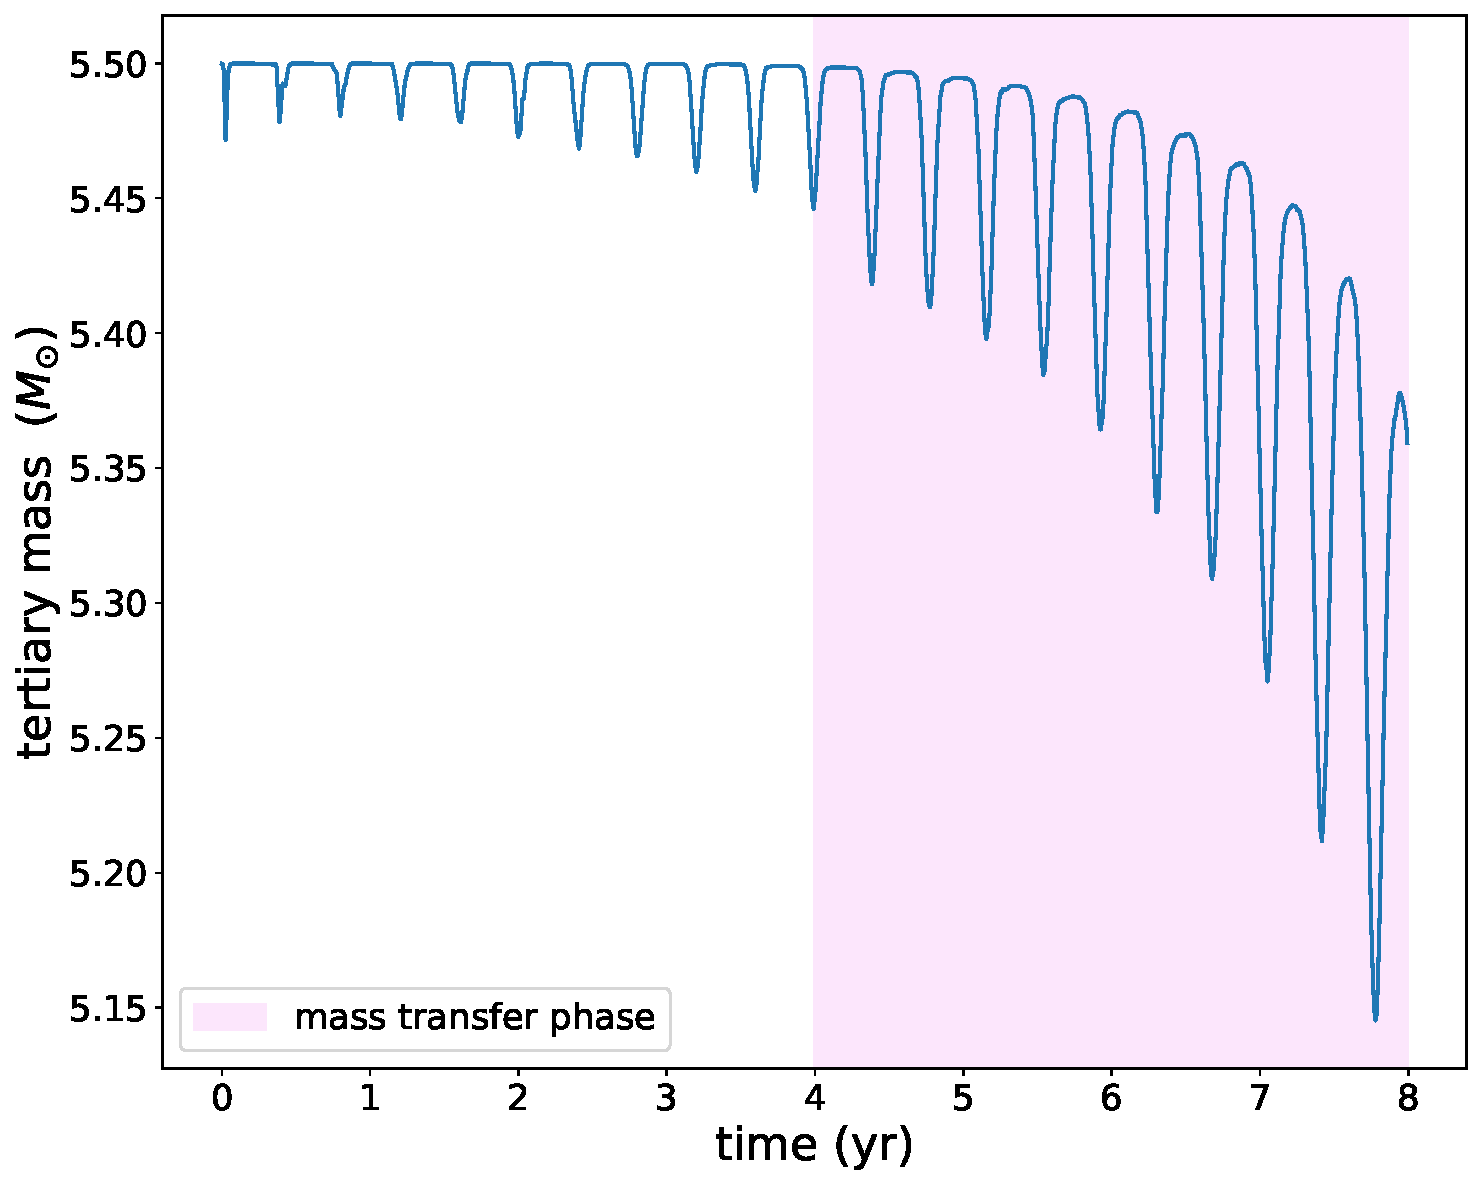
\includegraphics[width=0.85\textwidth]{Thesis/graphs/inc_00/accretion_inc_00_mass_loss.pdf}
    \caption{The evolution of the tertiary's mass.}
    \label{fig:accretion_inc_00_mass_loss}
\end{figure}
The mass evolution is periodic, modified by the outer orbit's periodicity, where $P_{out} = 145.5$ day or $P_{out} \approx 0.4$ yr. During the first four years of the simulation no remarkable mass transfer takes places. Gas particles escape from the gravitational well of the tertiary, close to the orbit's pericenter and later captured again, as the giant moves towards the orbit's apocenter, see subfigure in \cref{fig:accretion_inc_00_mass_loss}. In short, the tertiary experience a series of significant periodic distortions of its spherical symmetry, but the giant's mass remains the same.

Significant mass transfer from the tertiary towards the inner binary begins at $t \approx 4$ yr. As a result, this is the time period that is relevant for studying the effect of mass transfer on the evolution of the system. The mass transfer from the outer giant is periodic. This is due to the slightly eccentric outer orbit, which causes the giant to overfill its Roche lobe close to the orbit's pericenter, but after moving away from it, the star detaches from its Roche lobe, to re-establish \ac{rlof} when it reaches pericenter again. 

In \cref{fig:simualtion_snapshots}, I present eight snapshots of the system's evolution during one outer orbital period between $t = 6.3 - 6.67$ yr. From top to bottom and left to right, the time interval between the snapshots is $\approx 0.05$ yr or $18.25$ day. At $t \approx 6.3$ yr the giant crosses the orbit's pericenter and soon after, at $t \approx 6.35$ yr, the mass transfer rate becomes maximum. As the giant approaches the orbit's apocenter, $t \approx 6.4$ yr, the mass transfer rate decreases. At $t \approx 6.45$ yr, the giant crosses the orbit's apocenter and soon after, at $t \approx 6.5$ yr, detaches from its Roche lobe, only to re-establish \ac{rlof} at $t \approx 6.65$ yr.
\newpage
\thispagestyle{empty}
\vspace{-5cm}
\begin{figure}[H]
\vspace{-3cm}
    \centering
    \begin{subfigure}[b]{0.47\textwidth}
        \centering
        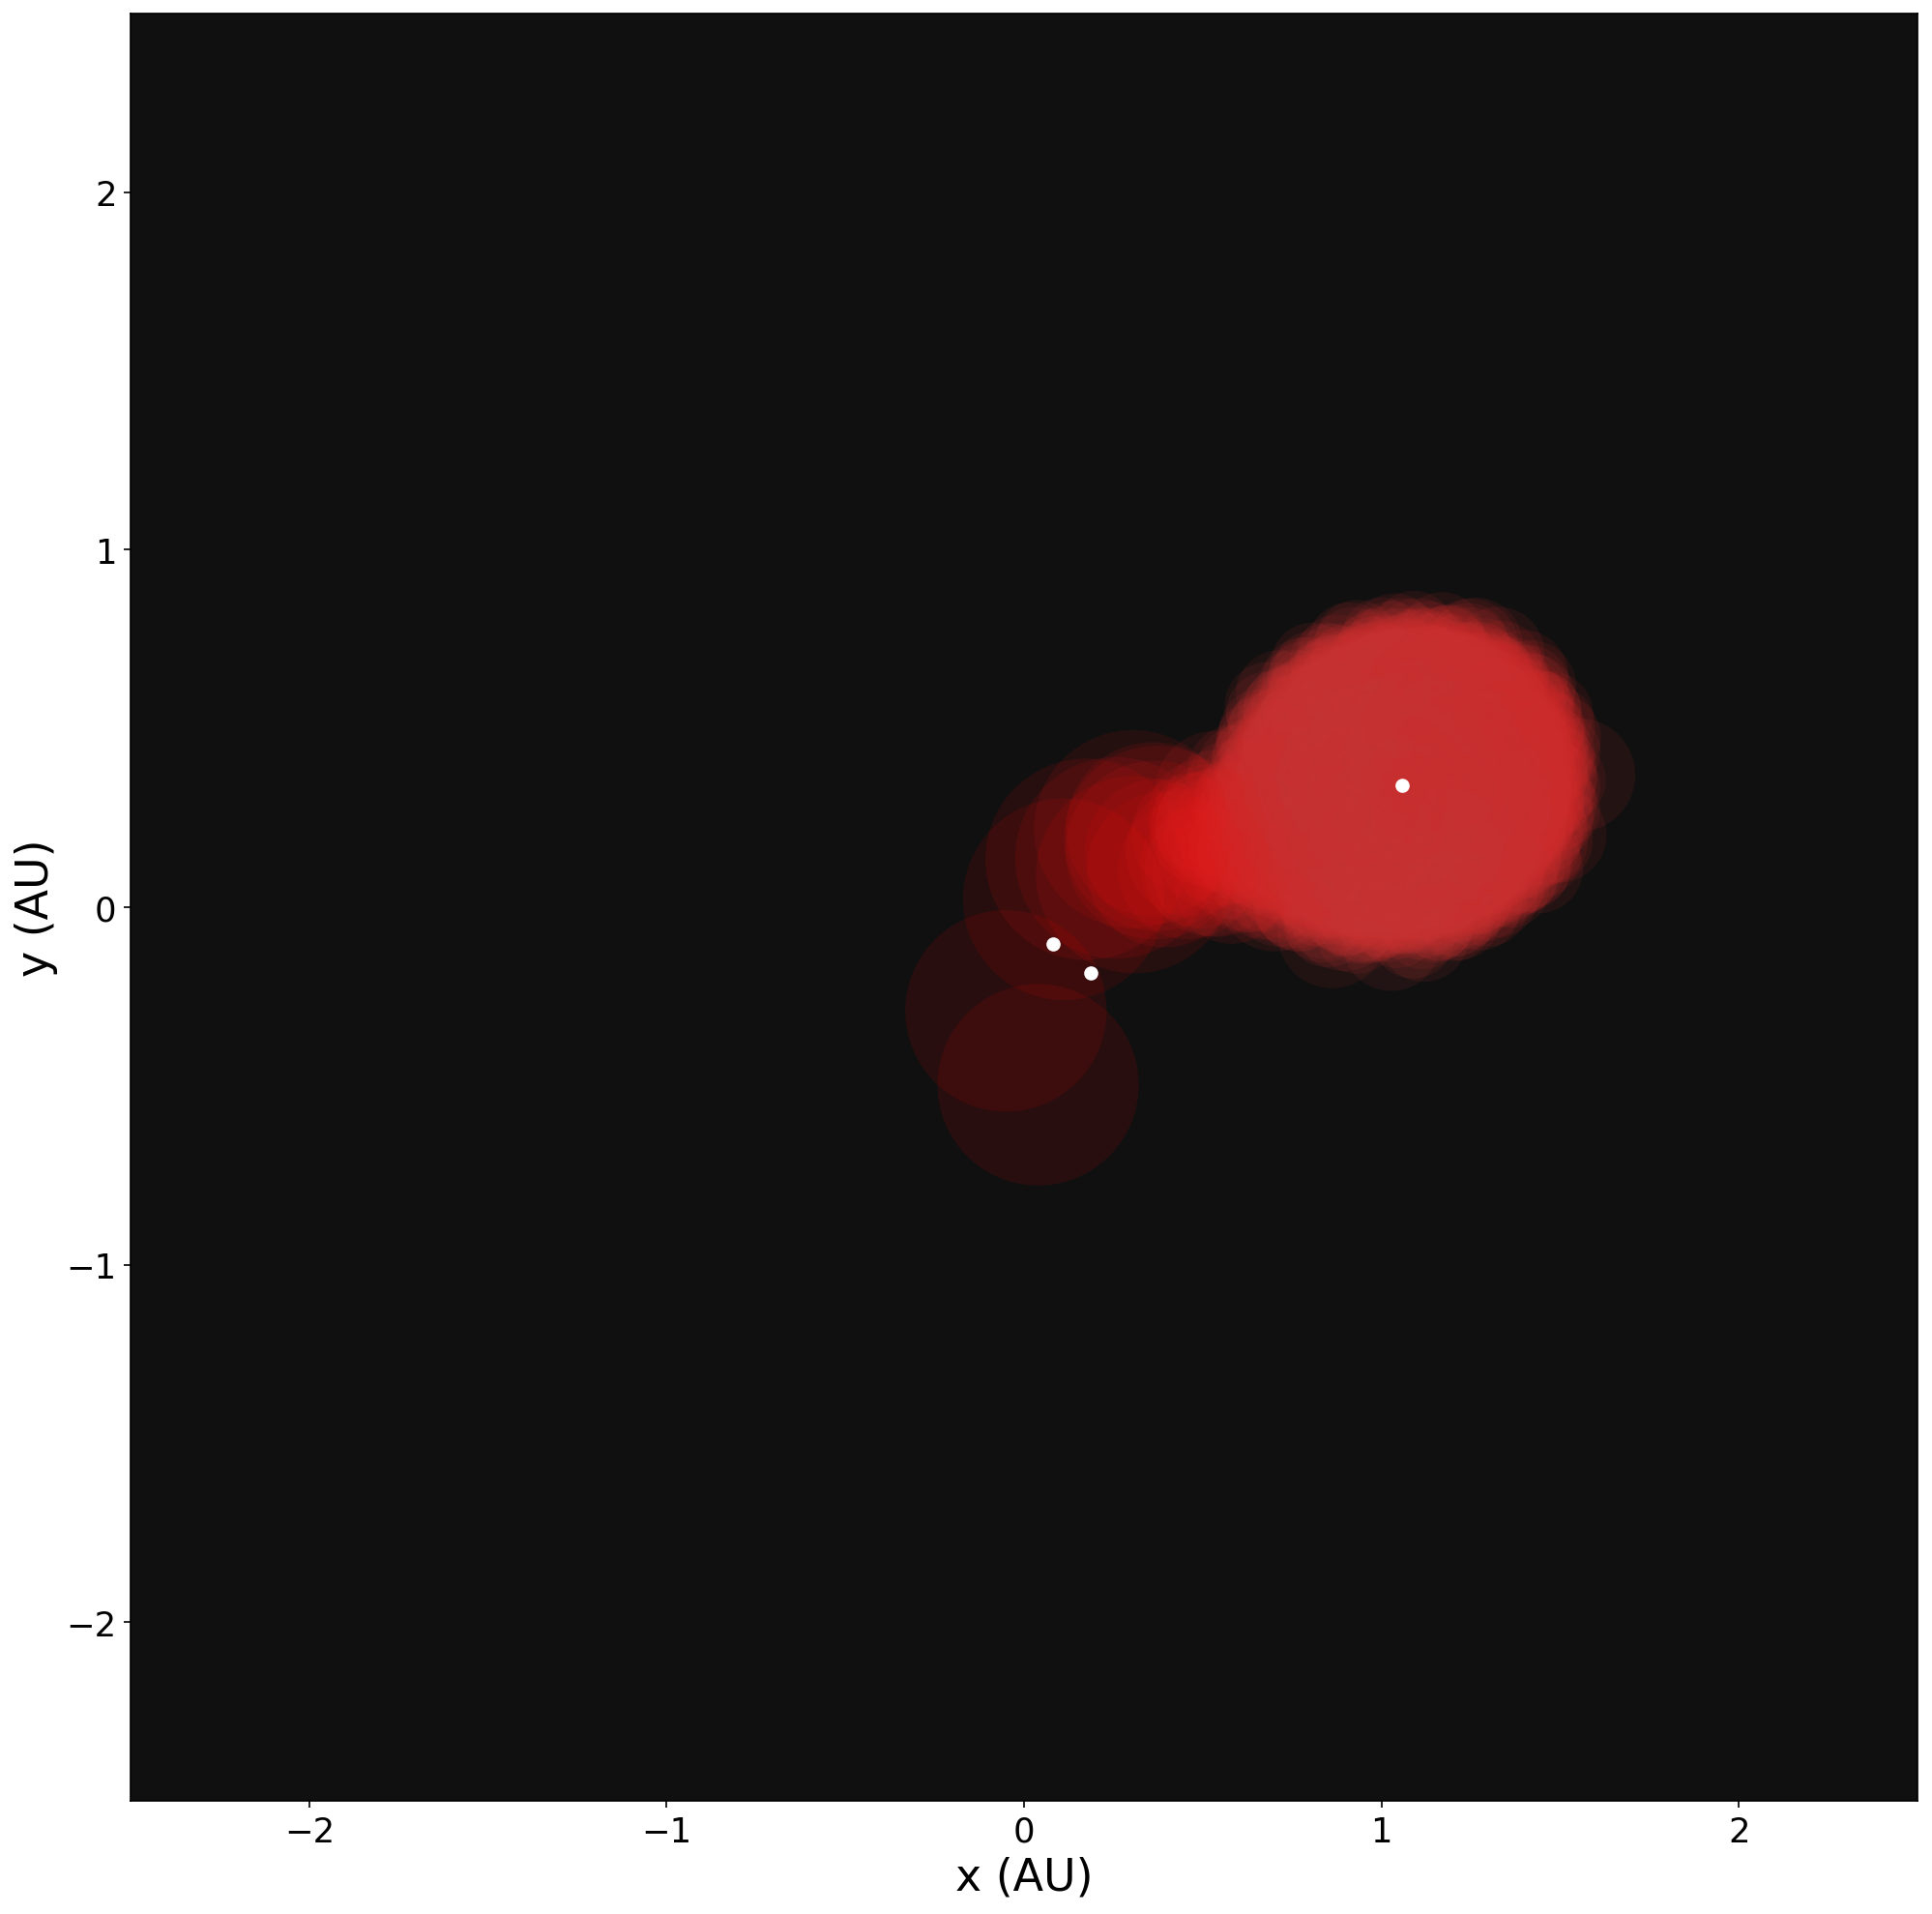
\includegraphics[width=\textwidth]{Thesis/graphs/snapshot_0022980.png}   
    \end{subfigure}
    \hfill
    \begin{subfigure}[b]{0.47\textwidth}  
        \centering 
        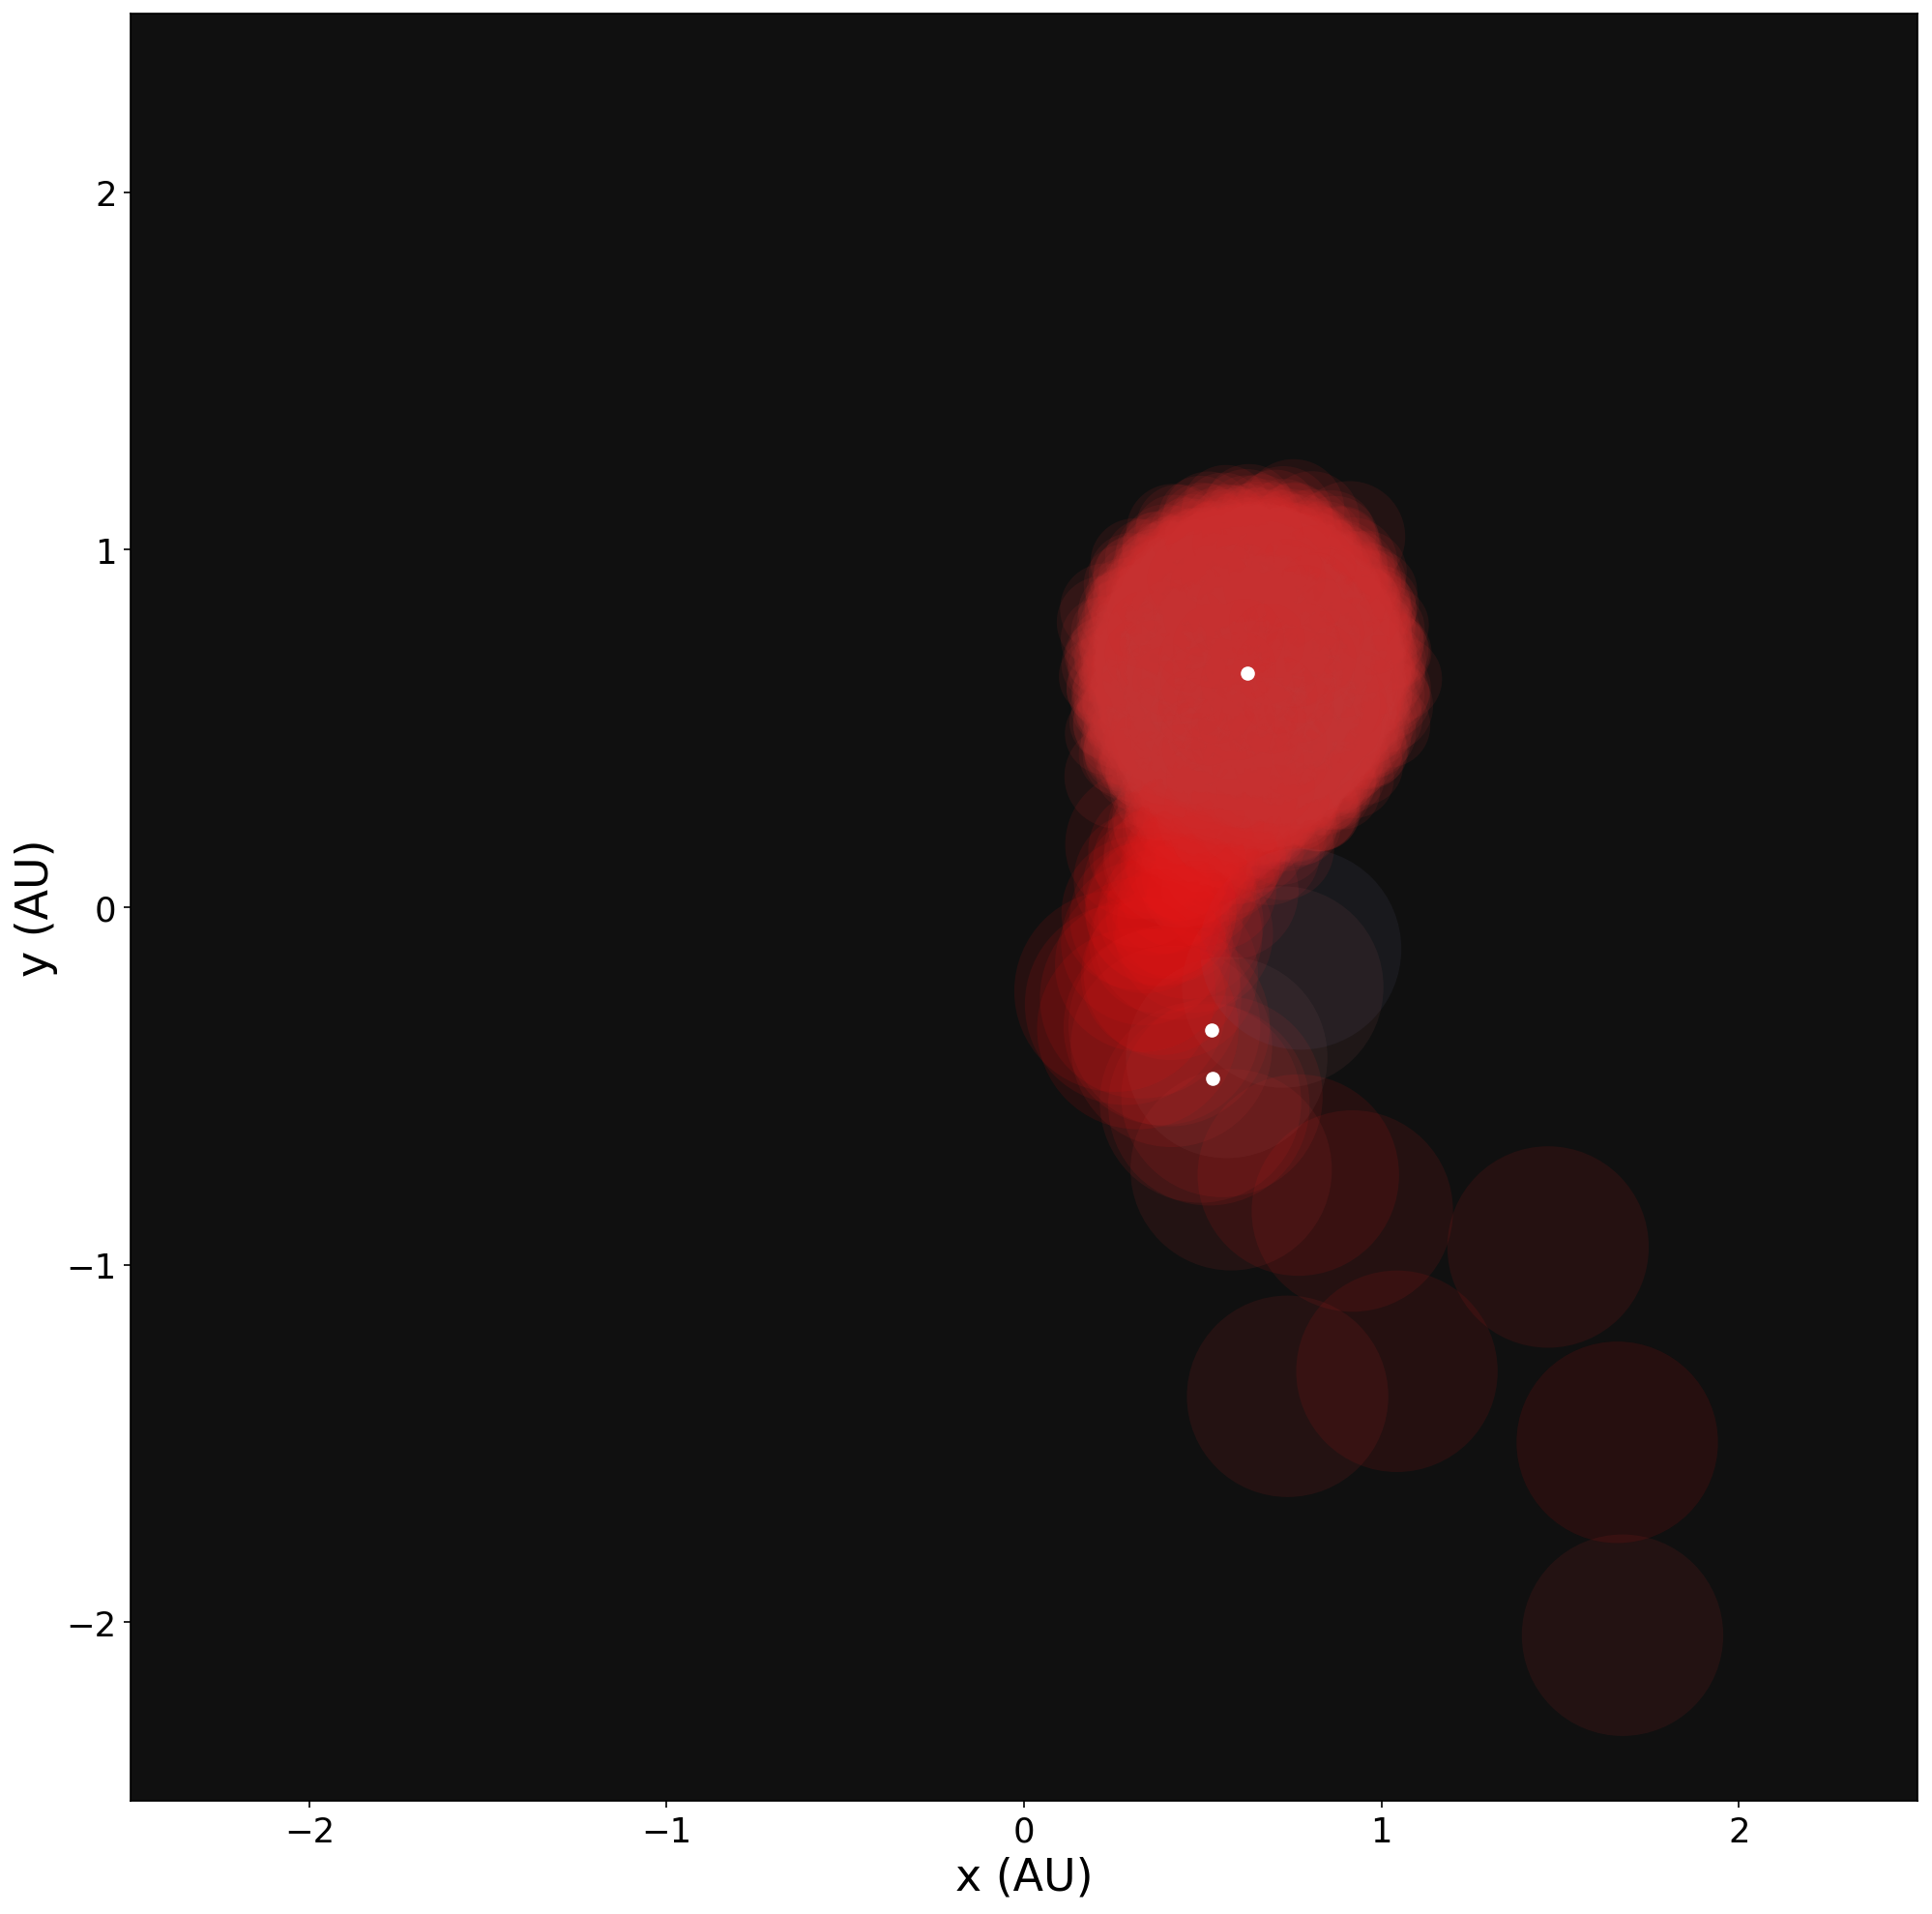
\includegraphics[width=\textwidth]{Thesis/graphs/snapshot_0023150.png}
    \end{subfigure}
    \hfill
    \begin{subfigure}[b]{0.47\textwidth}  
        \centering 
        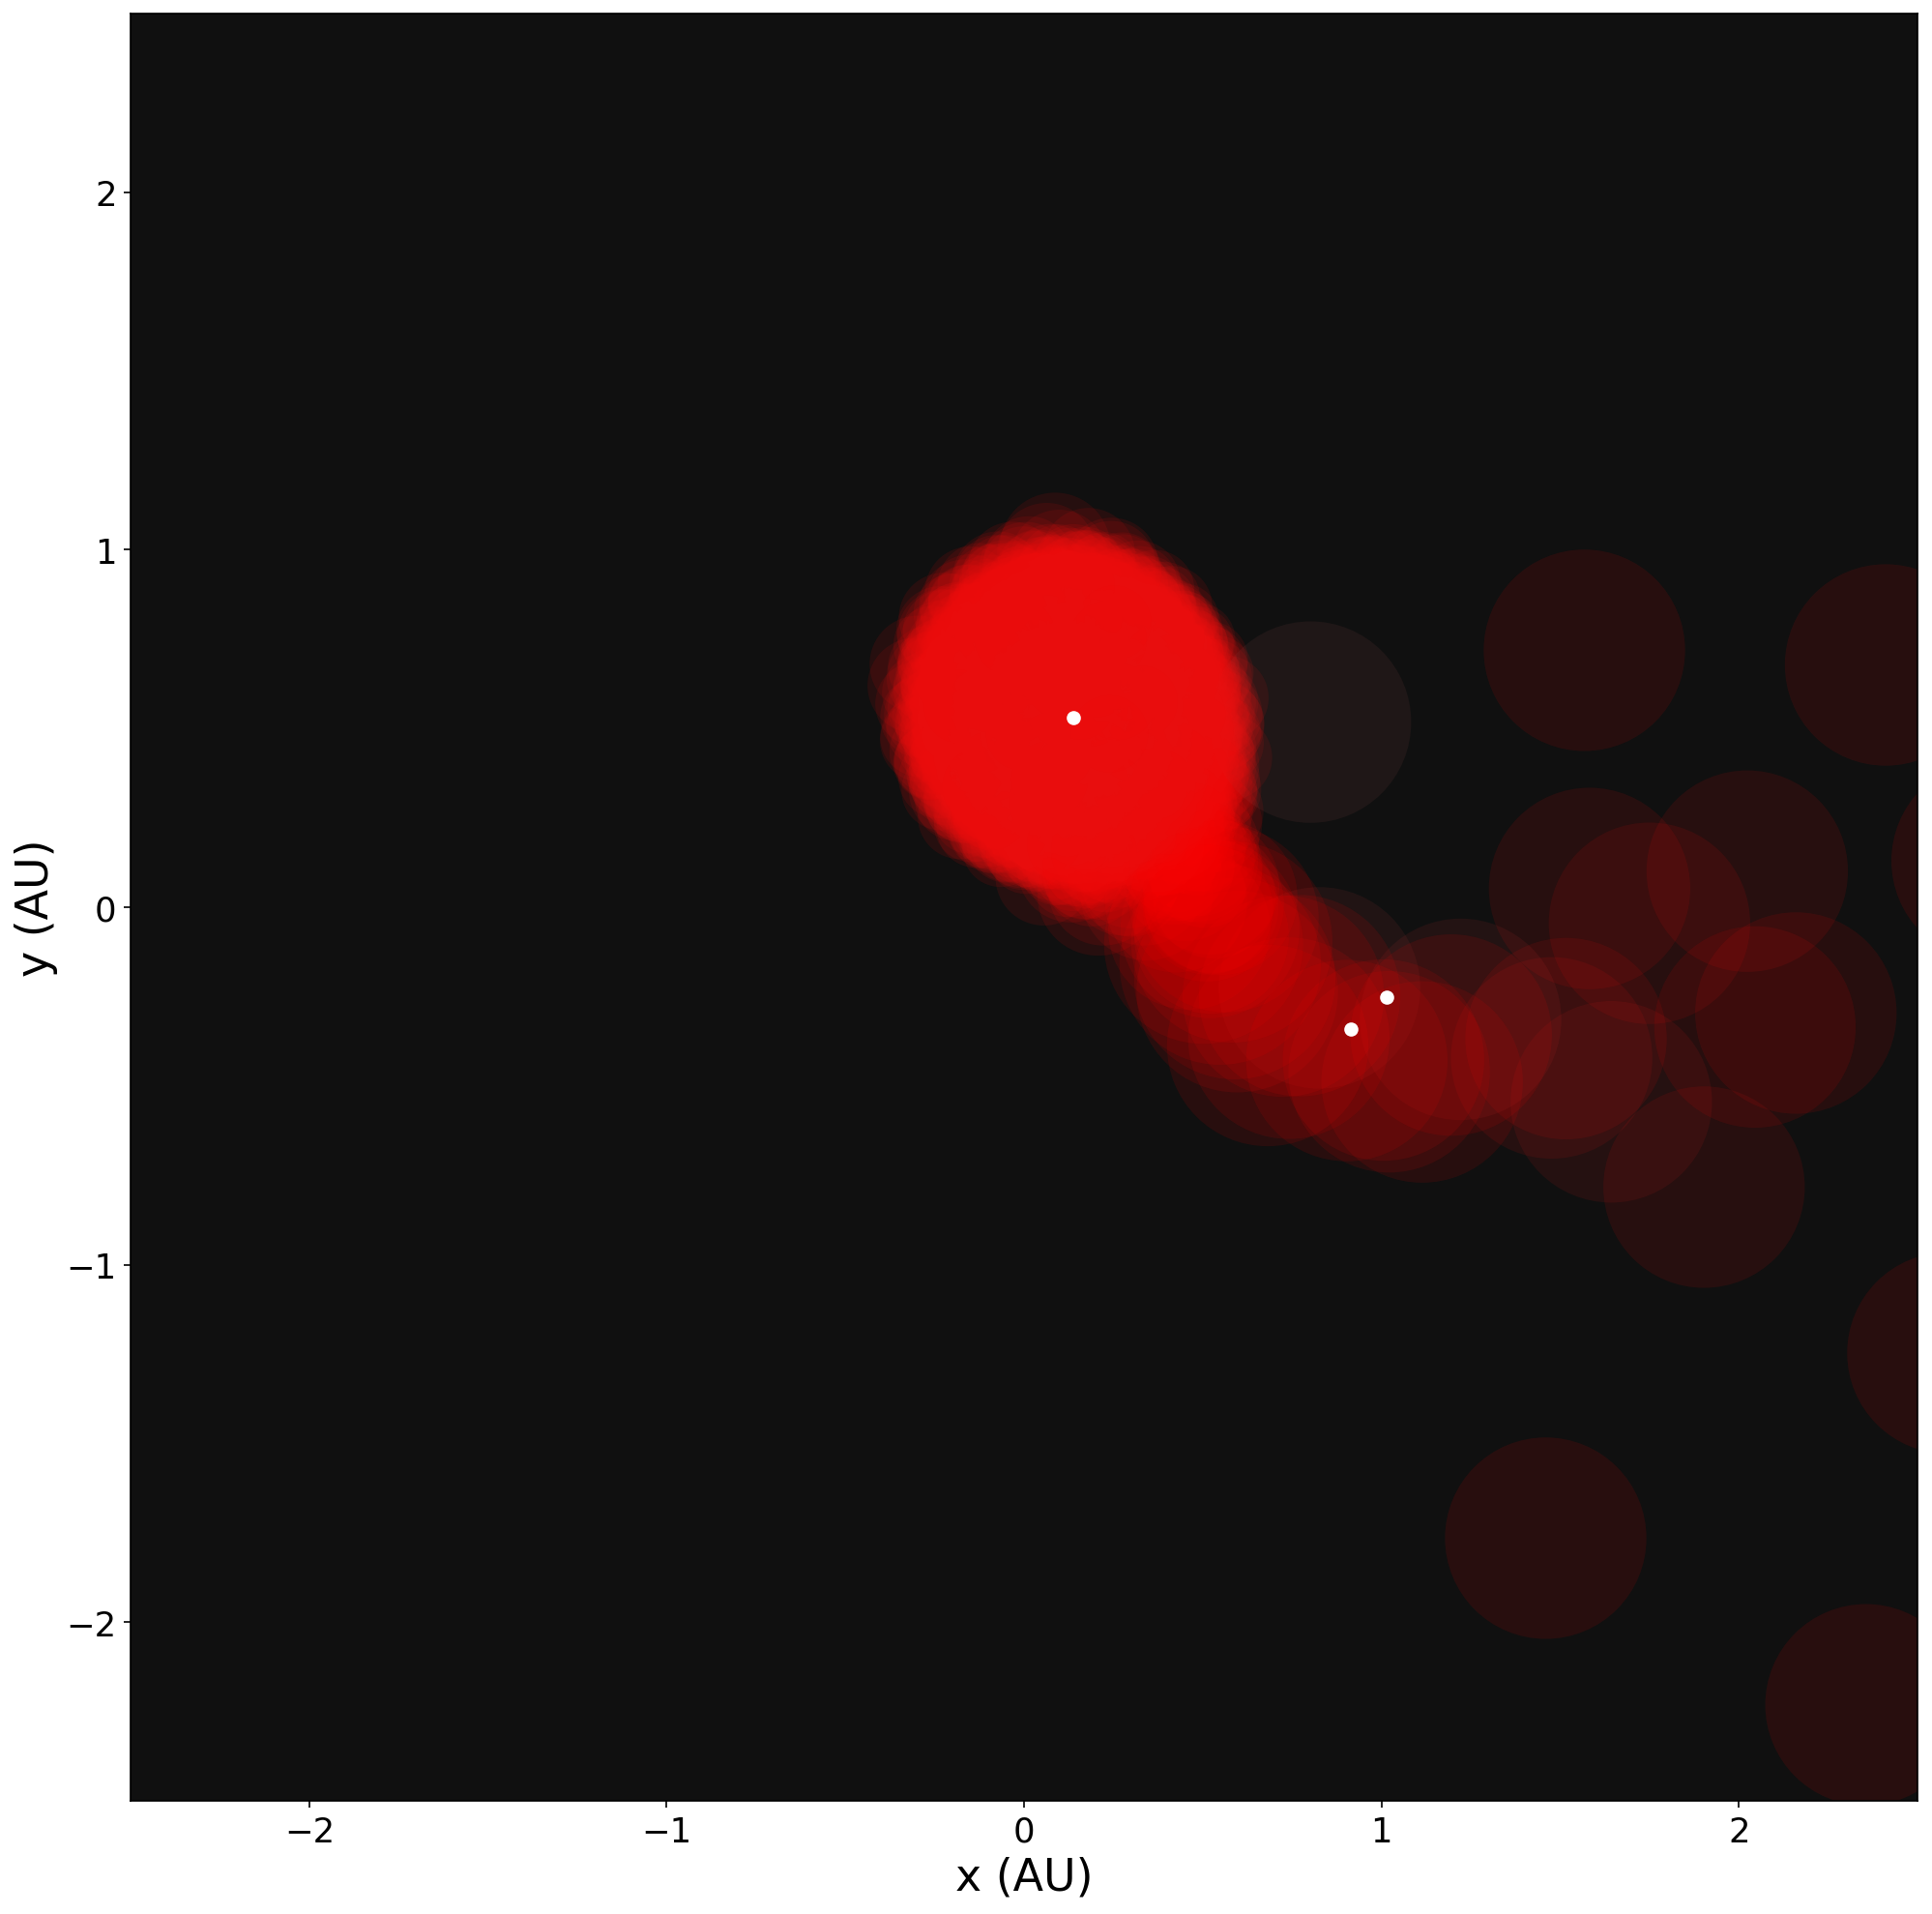
\includegraphics[width=\textwidth]{Thesis/graphs/snapshot_0023320.png}
    \end{subfigure}
    \hfill
    \begin{subfigure}[b]{0.47\textwidth}  
        \centering 
        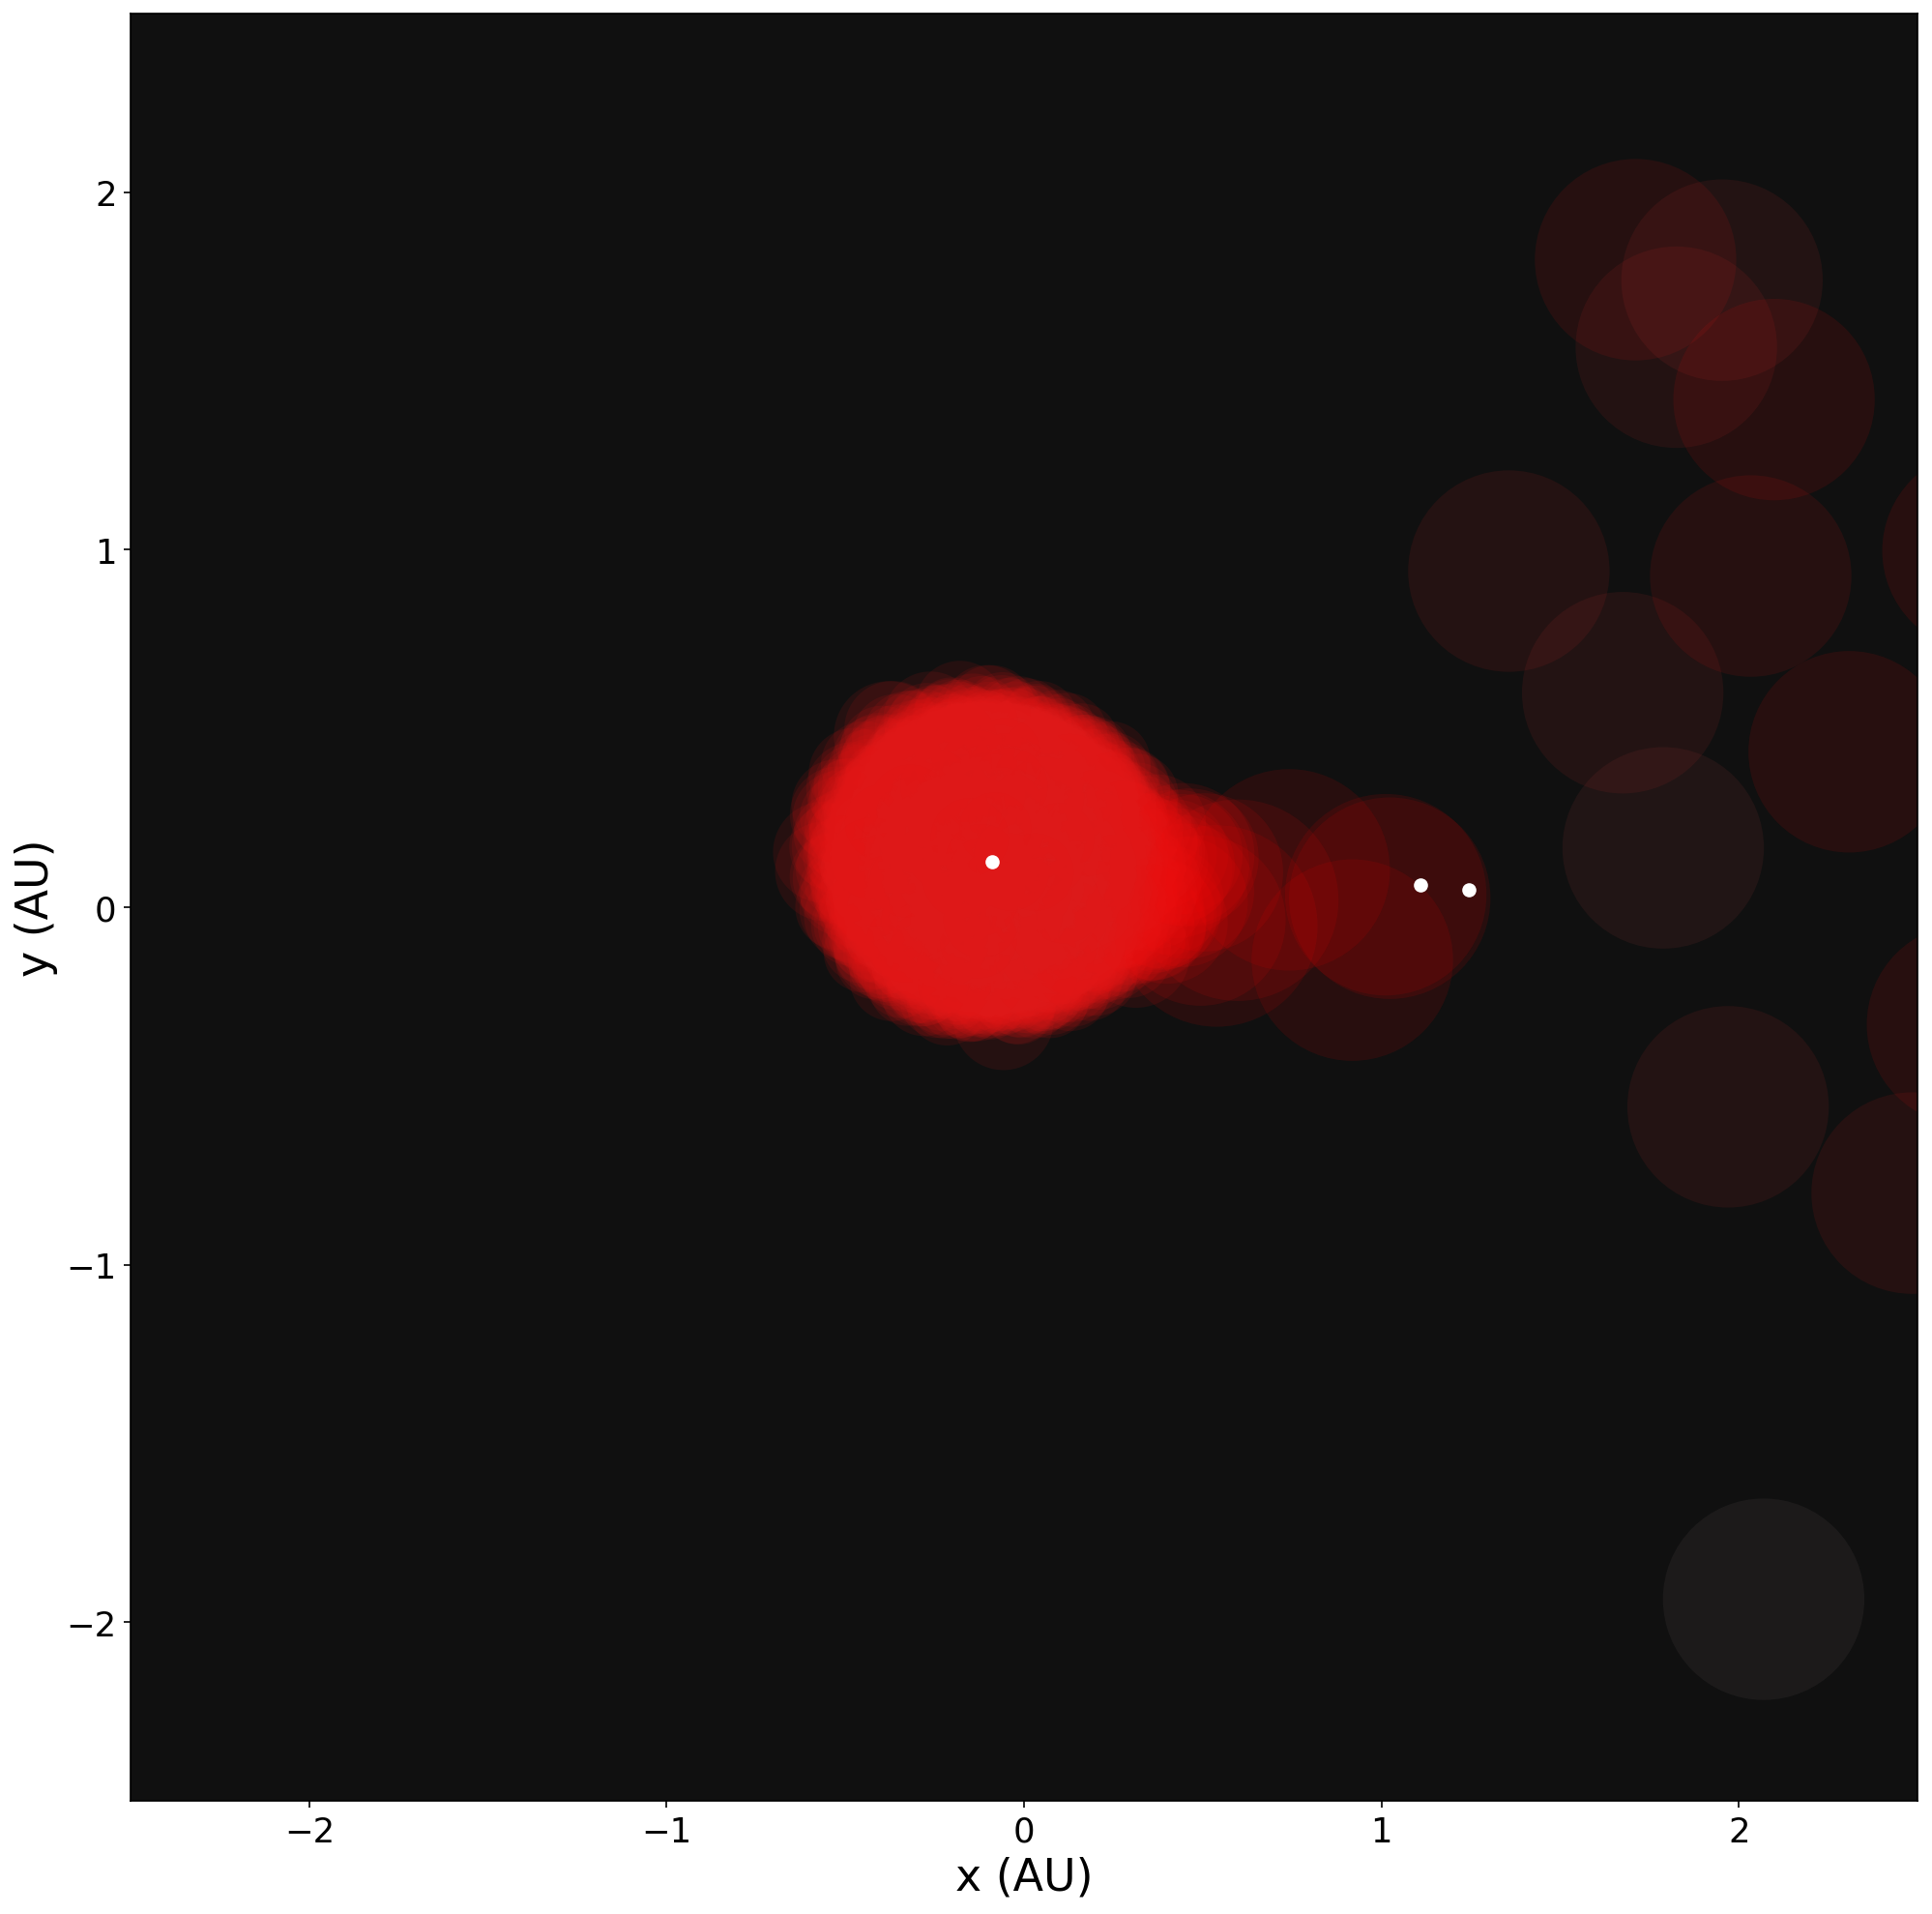
\includegraphics[width=\textwidth]{Thesis/graphs/snapshot_0023490.png}
    \end{subfigure}
    \hfill
    \begin{subfigure}[b]{0.47\textwidth}  
        \centering 
        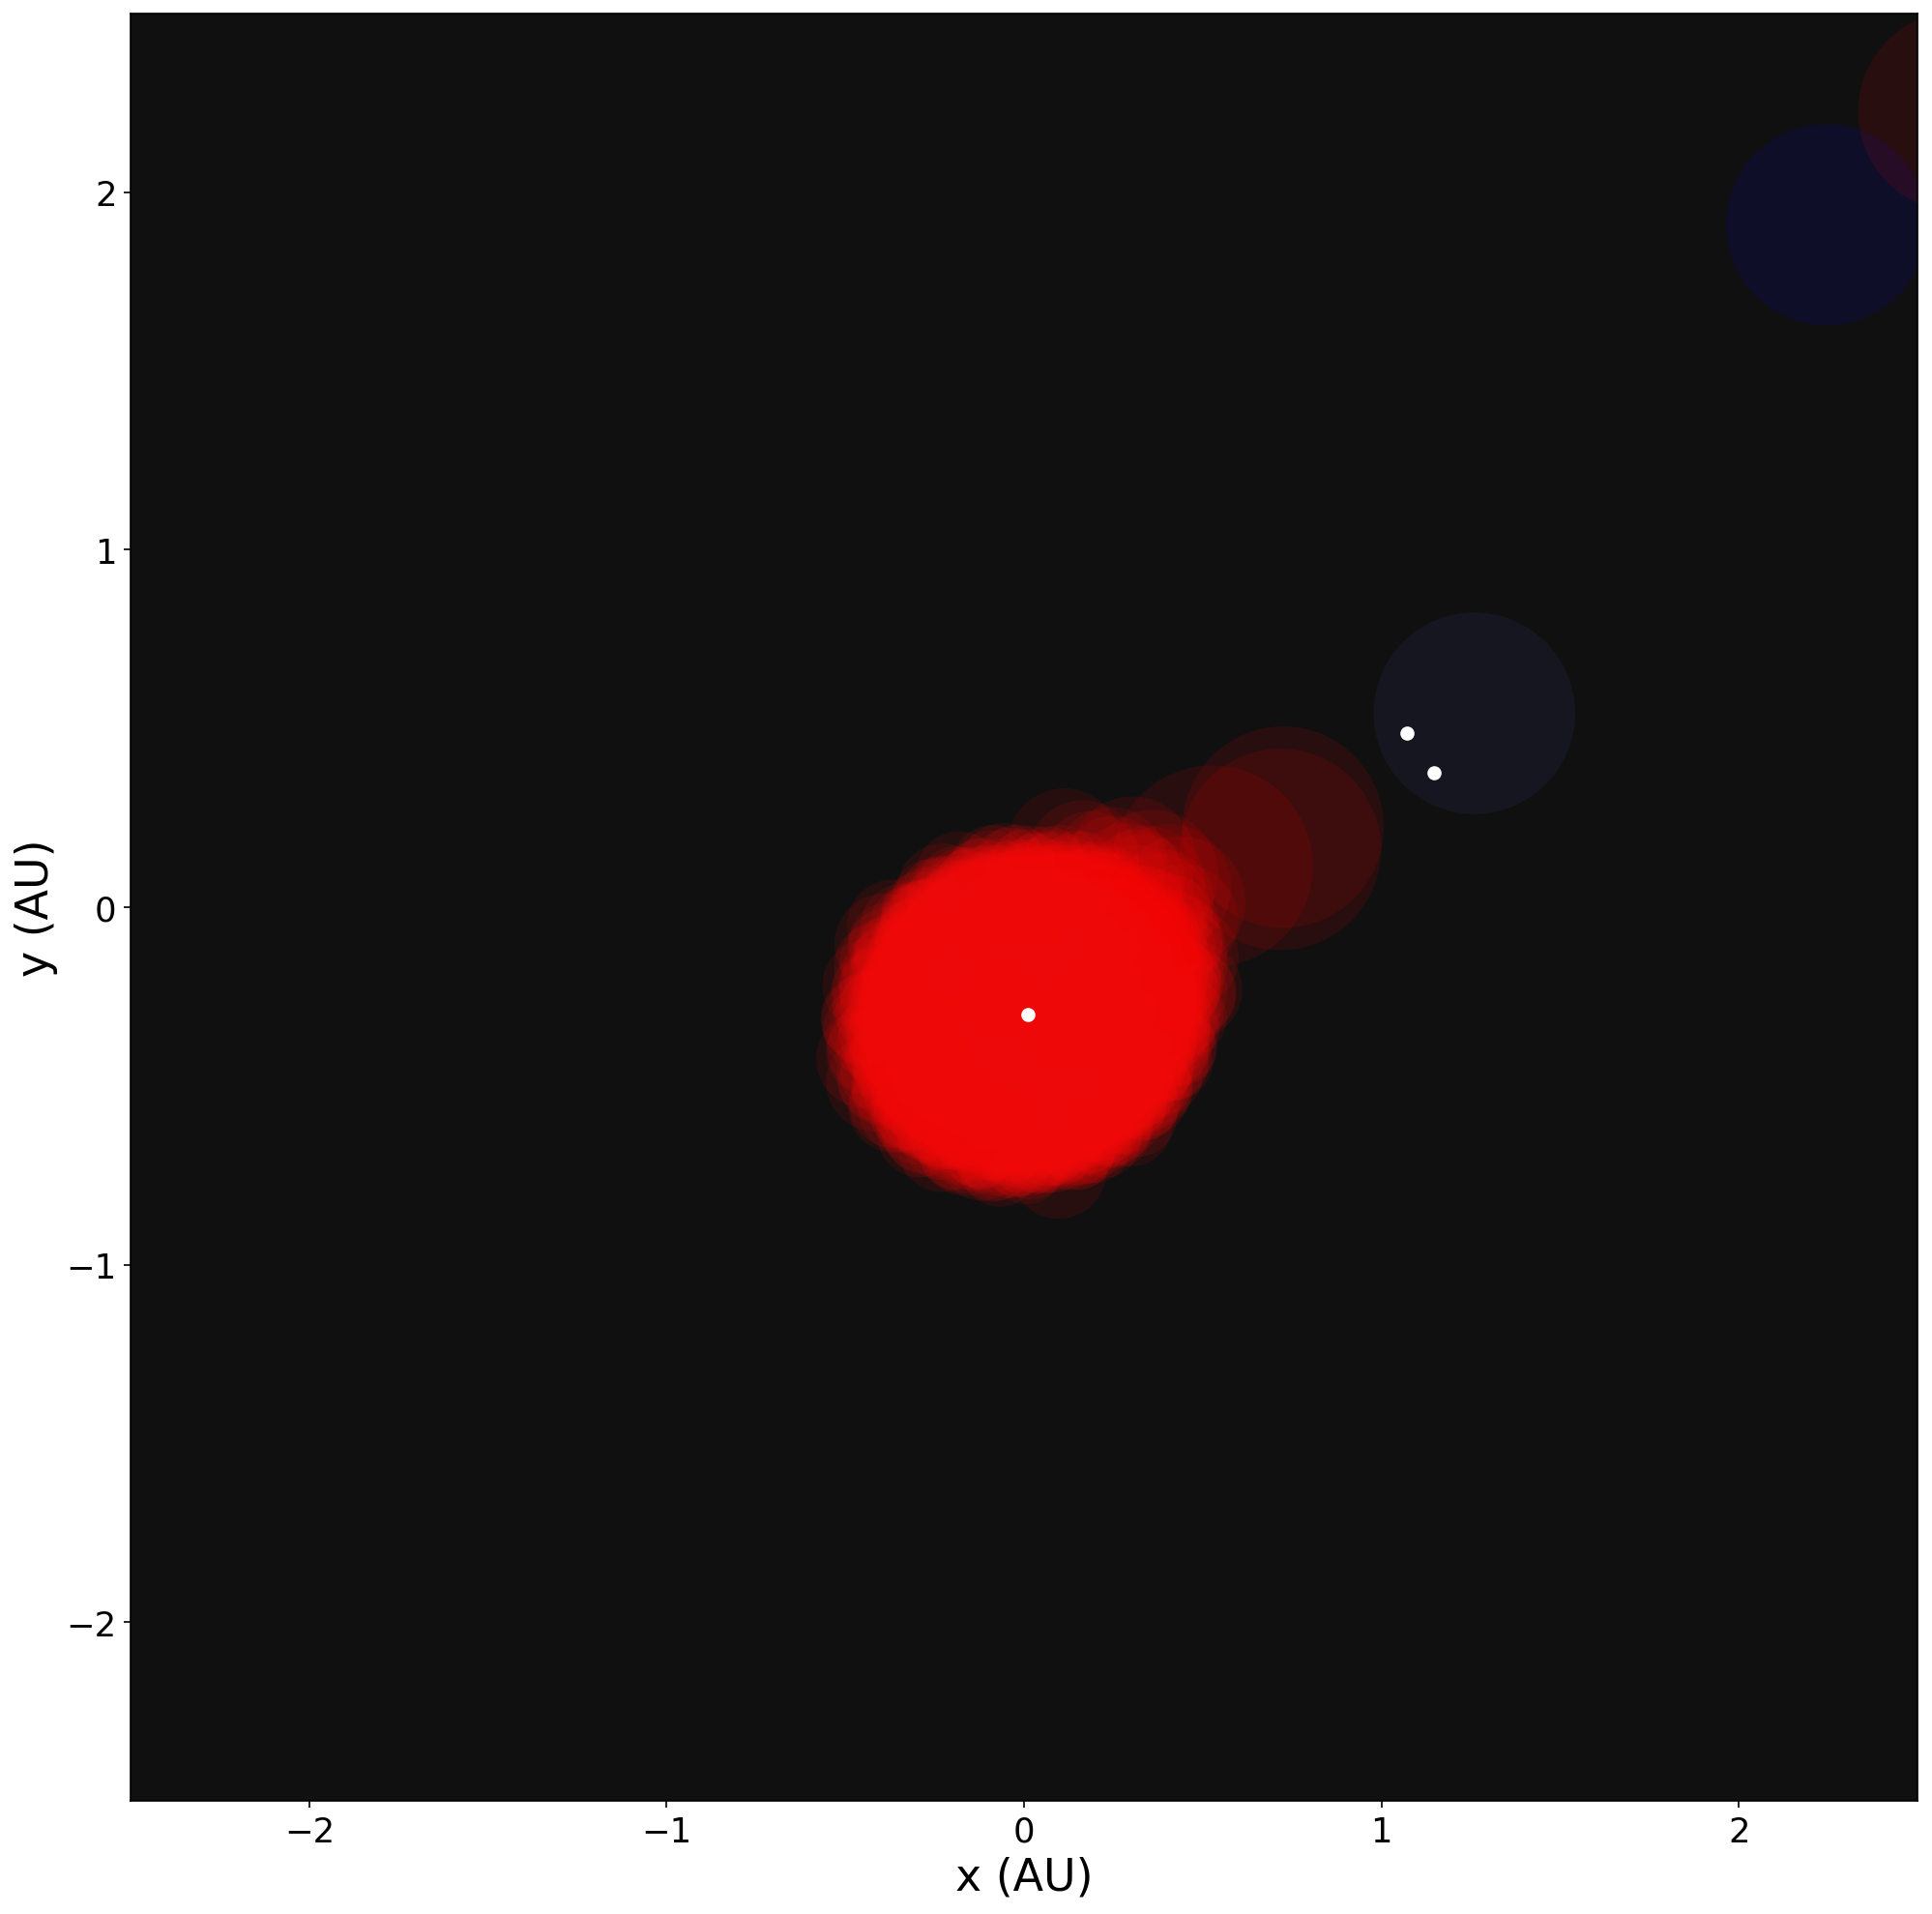
\includegraphics[width=\textwidth]{Thesis/graphs/snapshot_0023660.png}
    \end{subfigure}
    \hfill
    \begin{subfigure}[b]{0.47\textwidth}  
        \centering 
        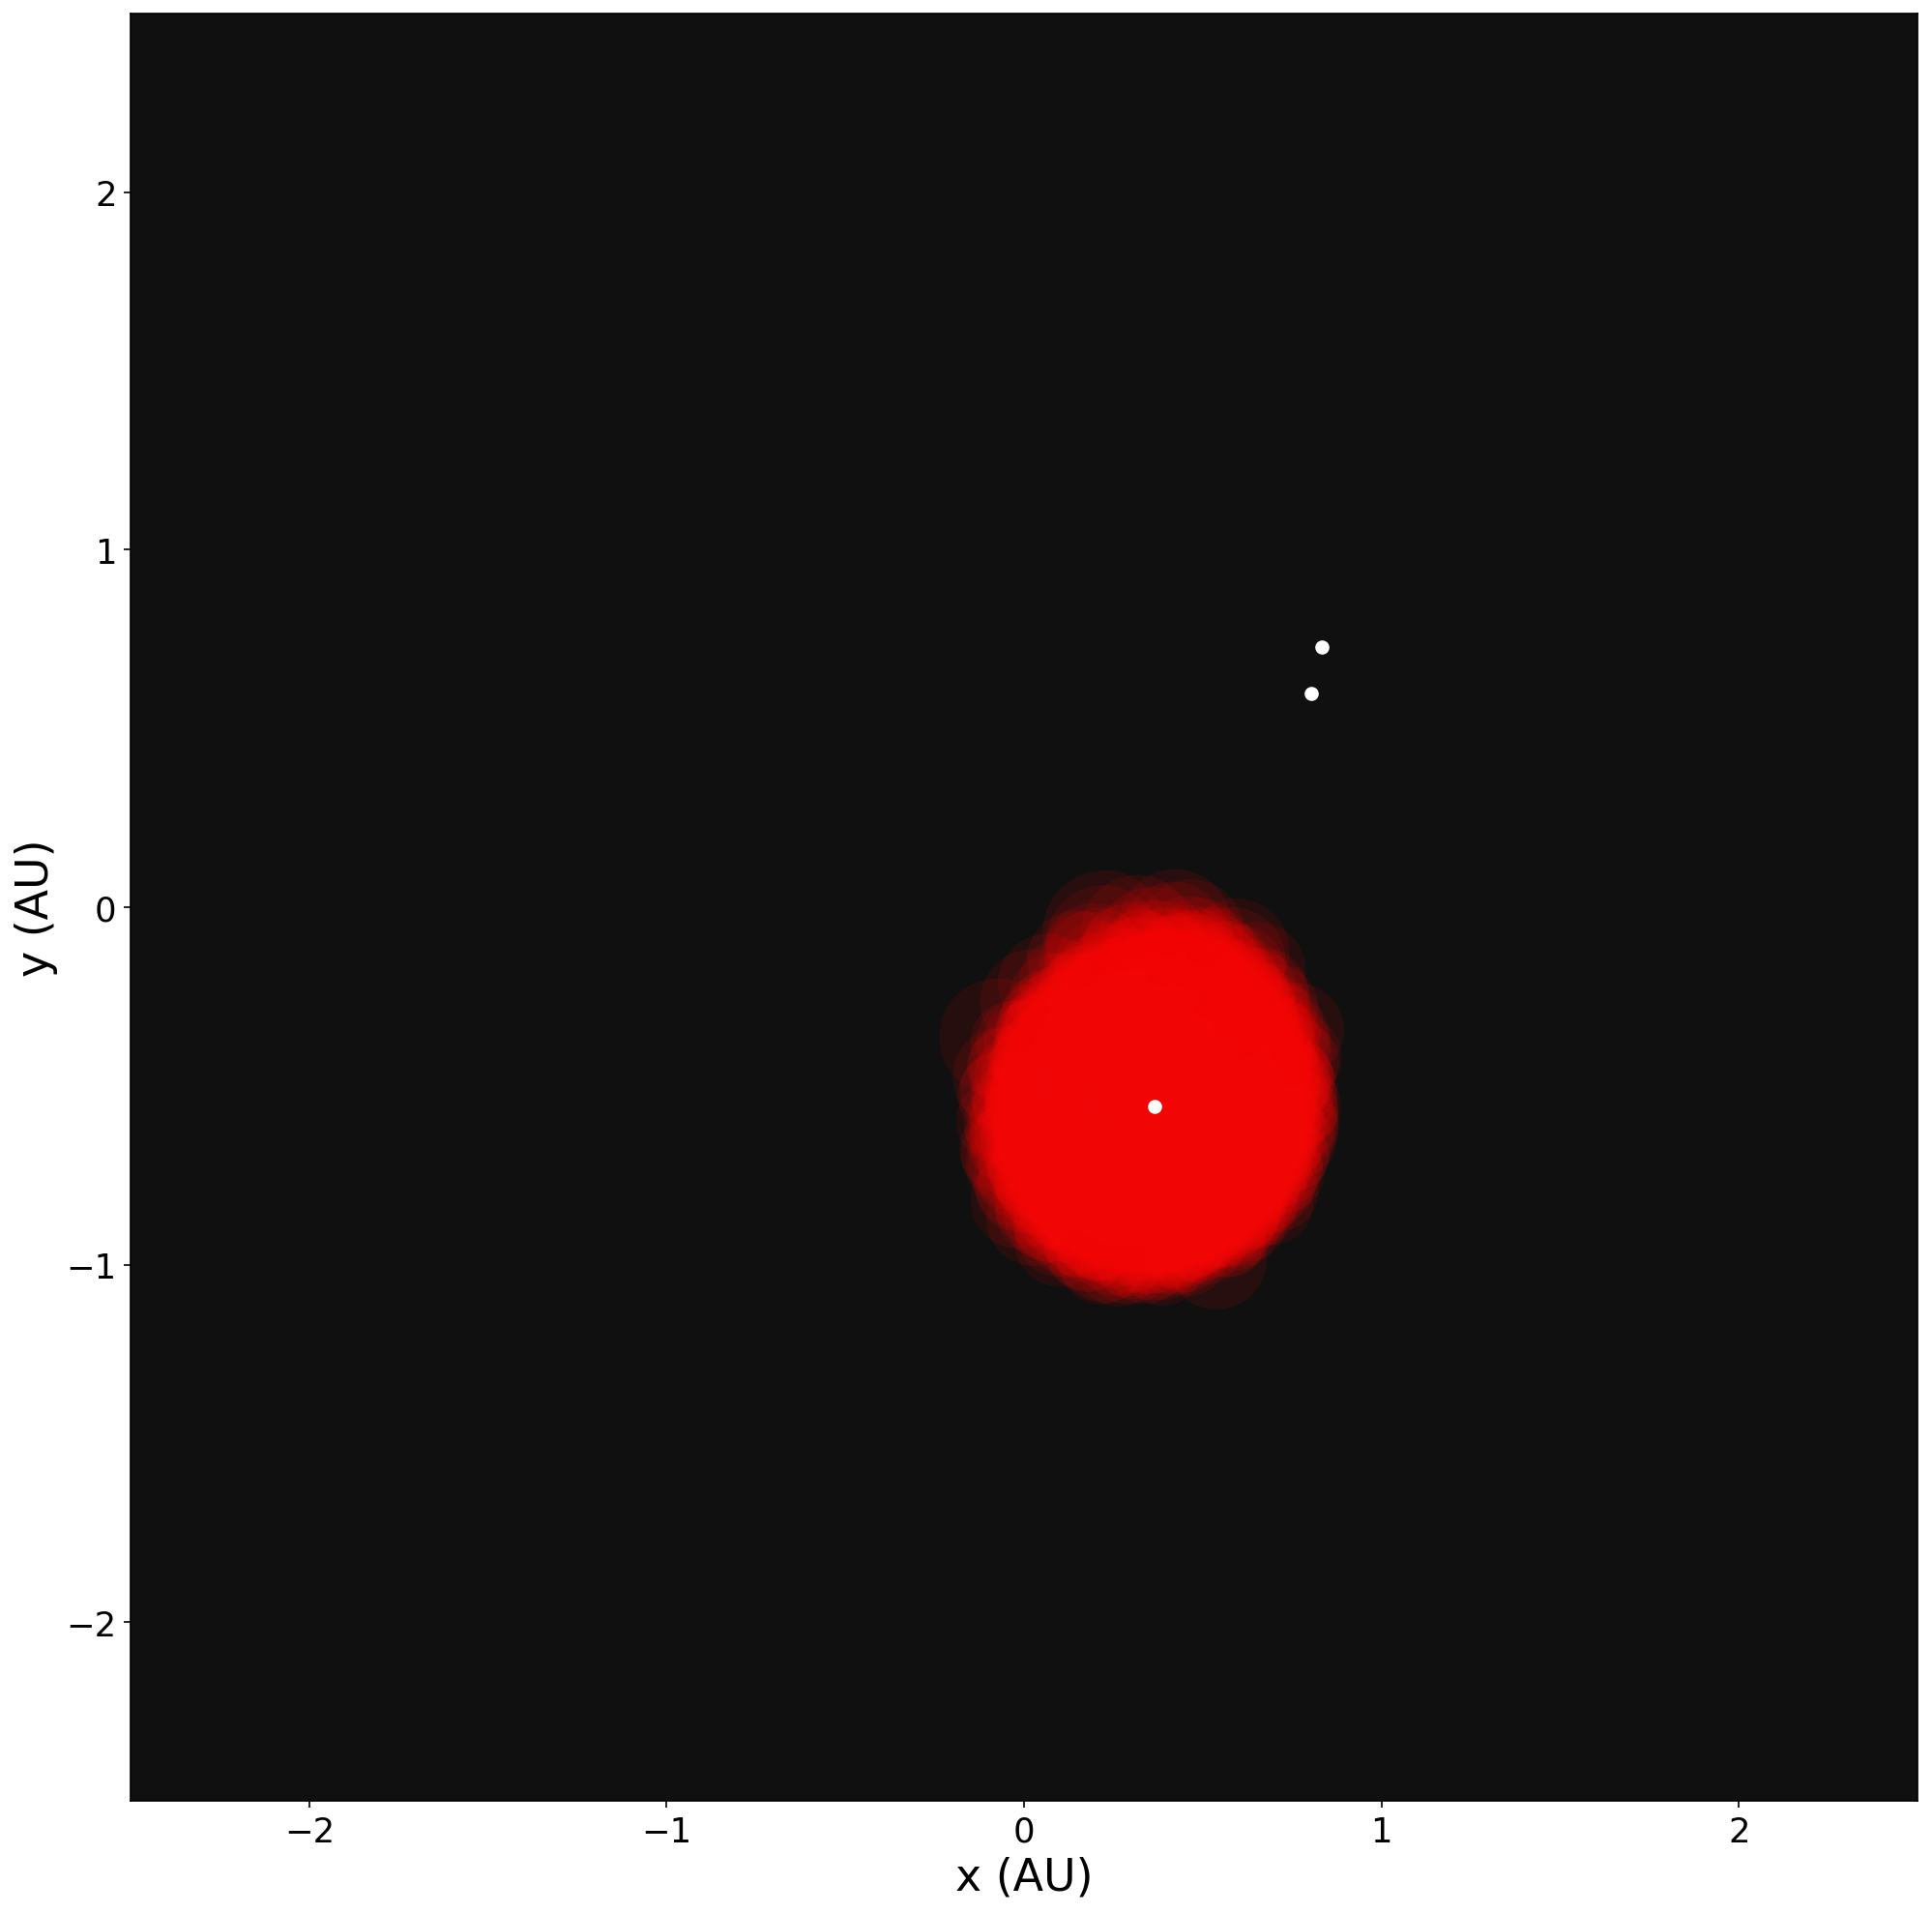
\includegraphics[width=\textwidth]{Thesis/graphs/snapshot_0023830.png}
    \end{subfigure}
    \hfill
    \begin{subfigure}[b]{0.47\textwidth}  
        \centering 
        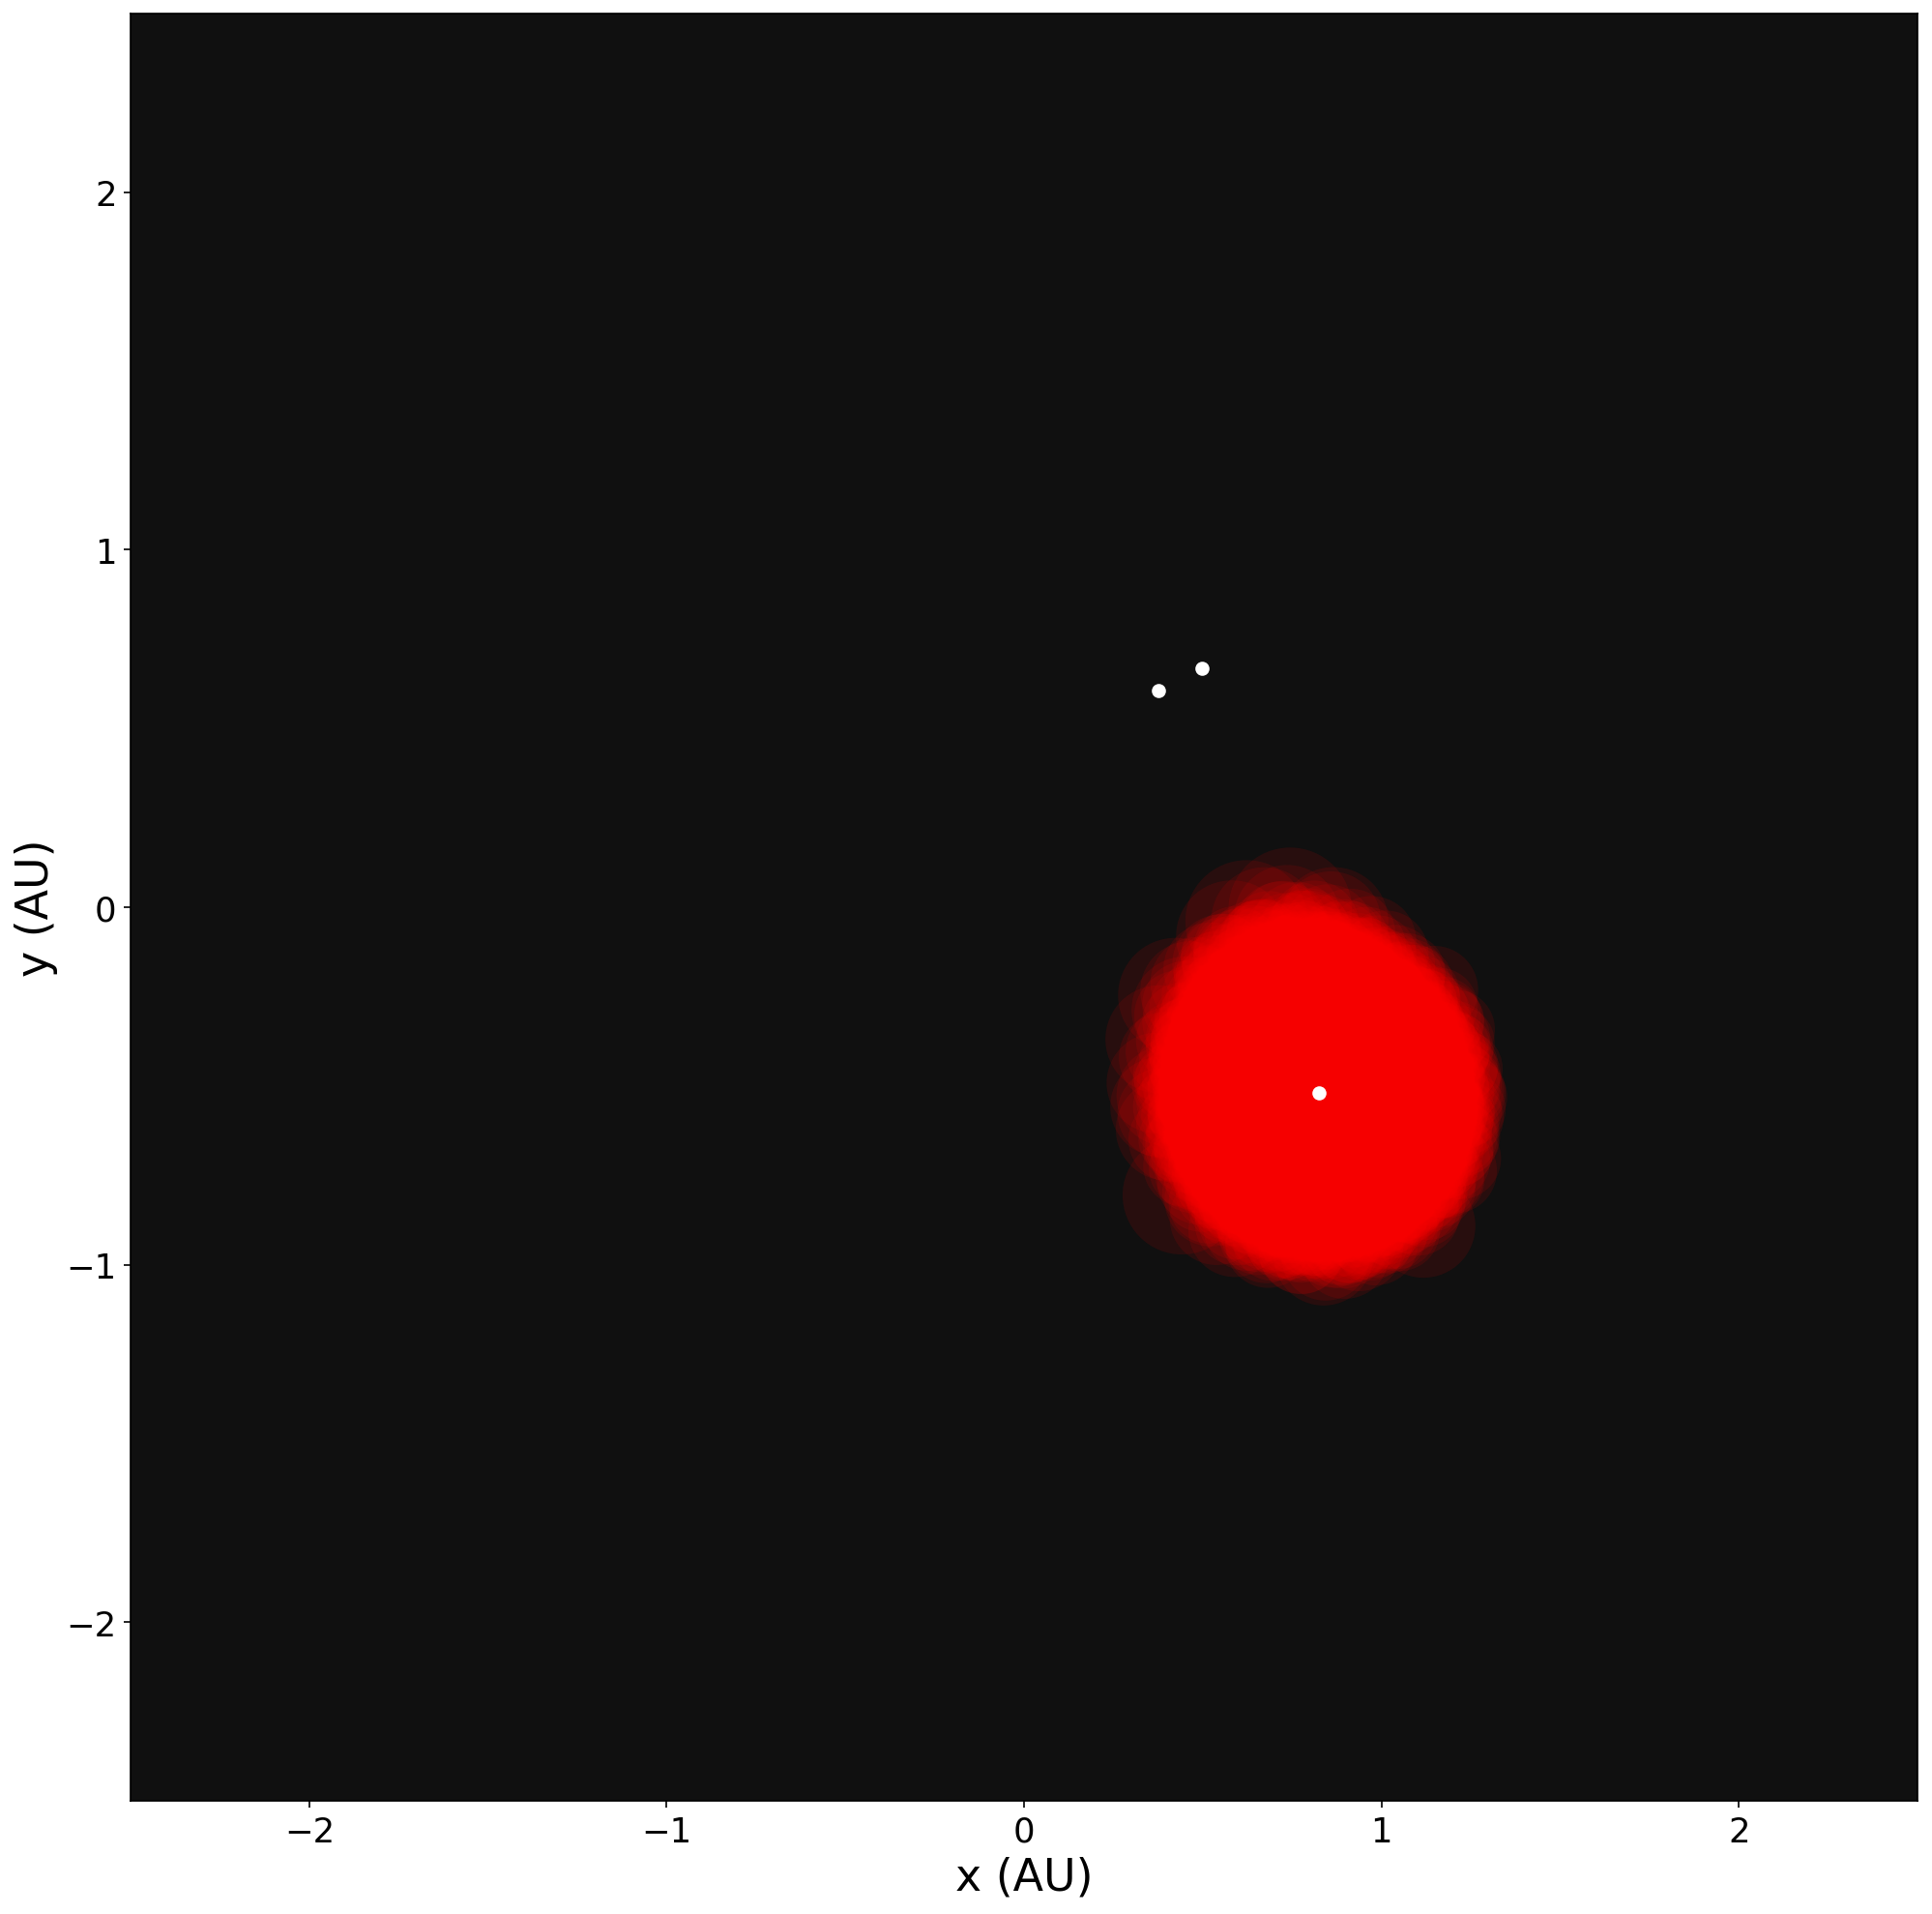
\includegraphics[width=\textwidth]{Thesis/graphs/snapshot_0024000.png}
    \end{subfigure}
    \hfill
    \begin{subfigure}[b]{0.47\textwidth}  
        \centering 
        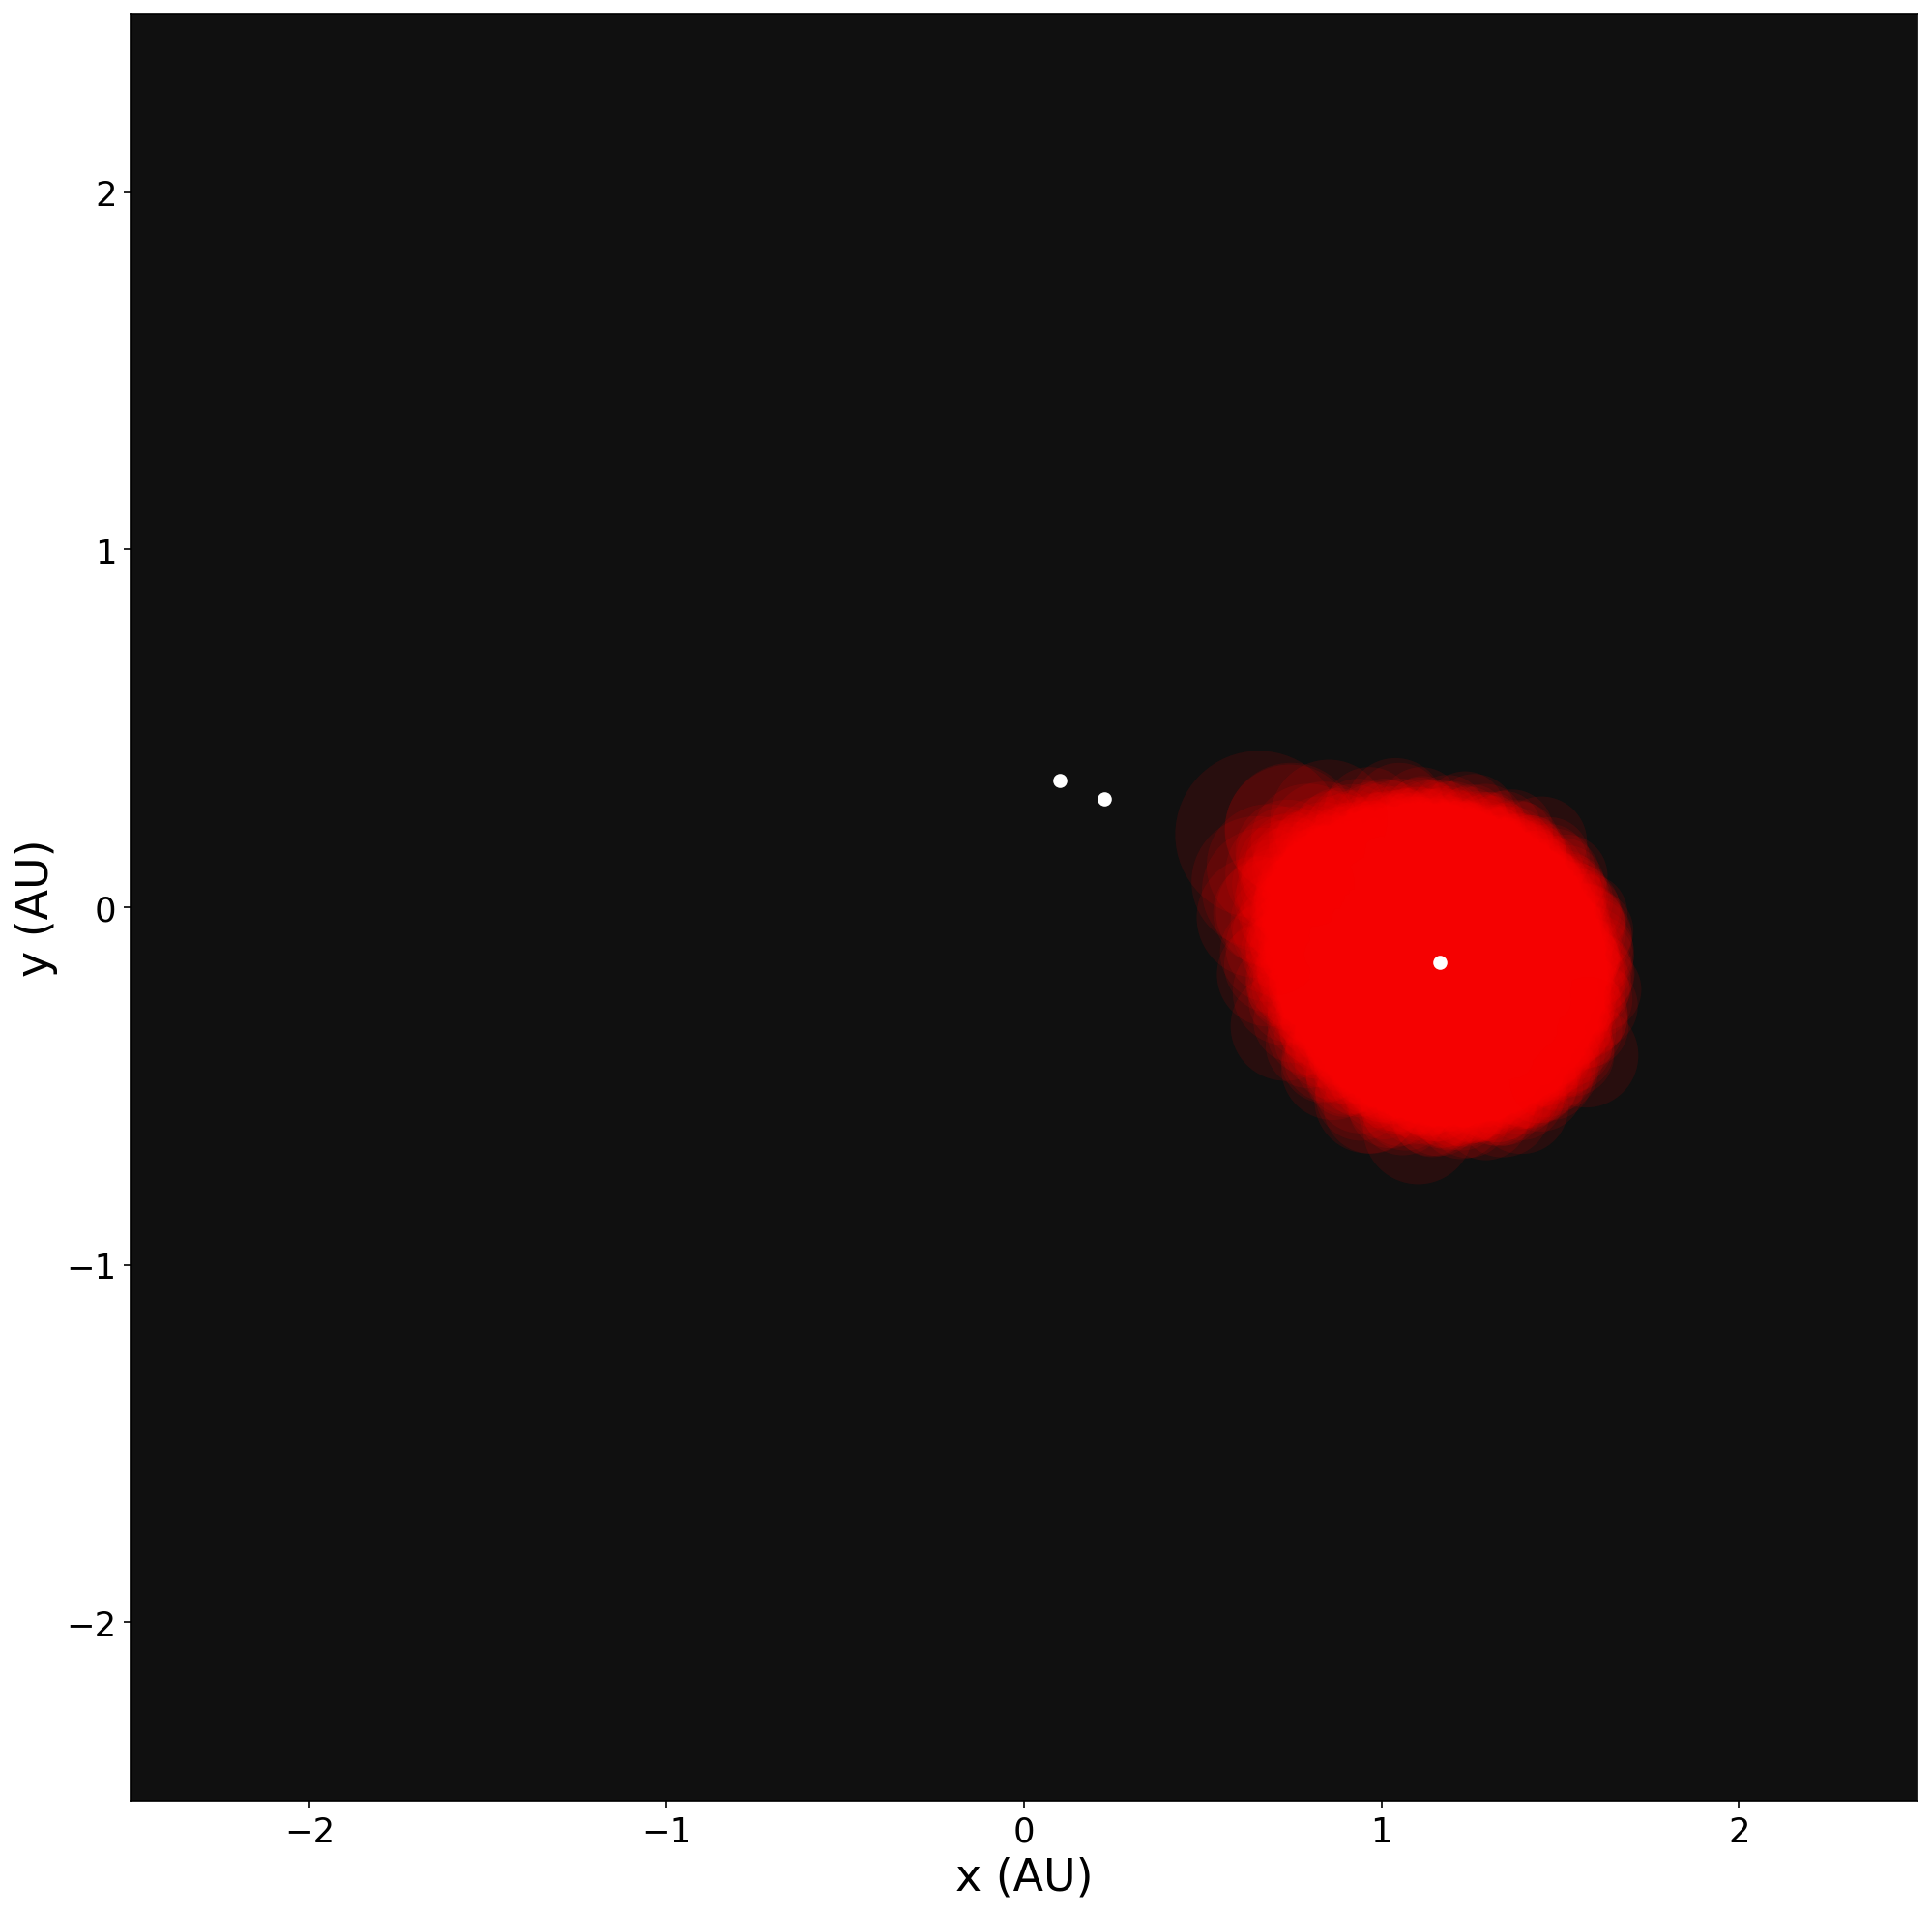
\includegraphics[width=\textwidth]{Thesis/graphs/snapshot_0024170.png}
    \end{subfigure}
    \caption{System snapshots, from top to bottom and left to right, at 6.3, 6.35, 6.4, 6.45, 6.5, 6.55, 6.6 and 6.65 yr. The white points are the purely gravitational particles representing the core and the inner binary components. The red points are the \ac{sph} particles representing the gas having an adaptive smoothing length.}
    \label{fig:simualtion_snapshots}
\end{figure}

I notice that, there is a significant delay between the moments of pericenter crossing and the maxima in mass transfer, see \cref{fig:simualtion_snapshots}, which is consistent with a study of \ac{rlof} in eccentric binaries \citep{lajoie2010mass}.

\subsection{Outer orbit}

In \cref{fig:accretion_inc_00_outer_semimajor_axis} and \cref{fig:accretion_inc_00_outer_ecc}, I present the evolution of the semi-major axis and eccentricity of the outer orbit, respectively. Additionally, \cref{fig:accretion_inc_00_inc} illustrates the evolution of the outer orbit's inclination relative to the inner orbit. During the simulation, the outer orbit shrinks, circularizes and remains in coplanarity with the inner orbit. However, the rates of change of the aforementioned orbital parameters alter as mass transfer begins.
\begin{figure}[H]
    \centering
    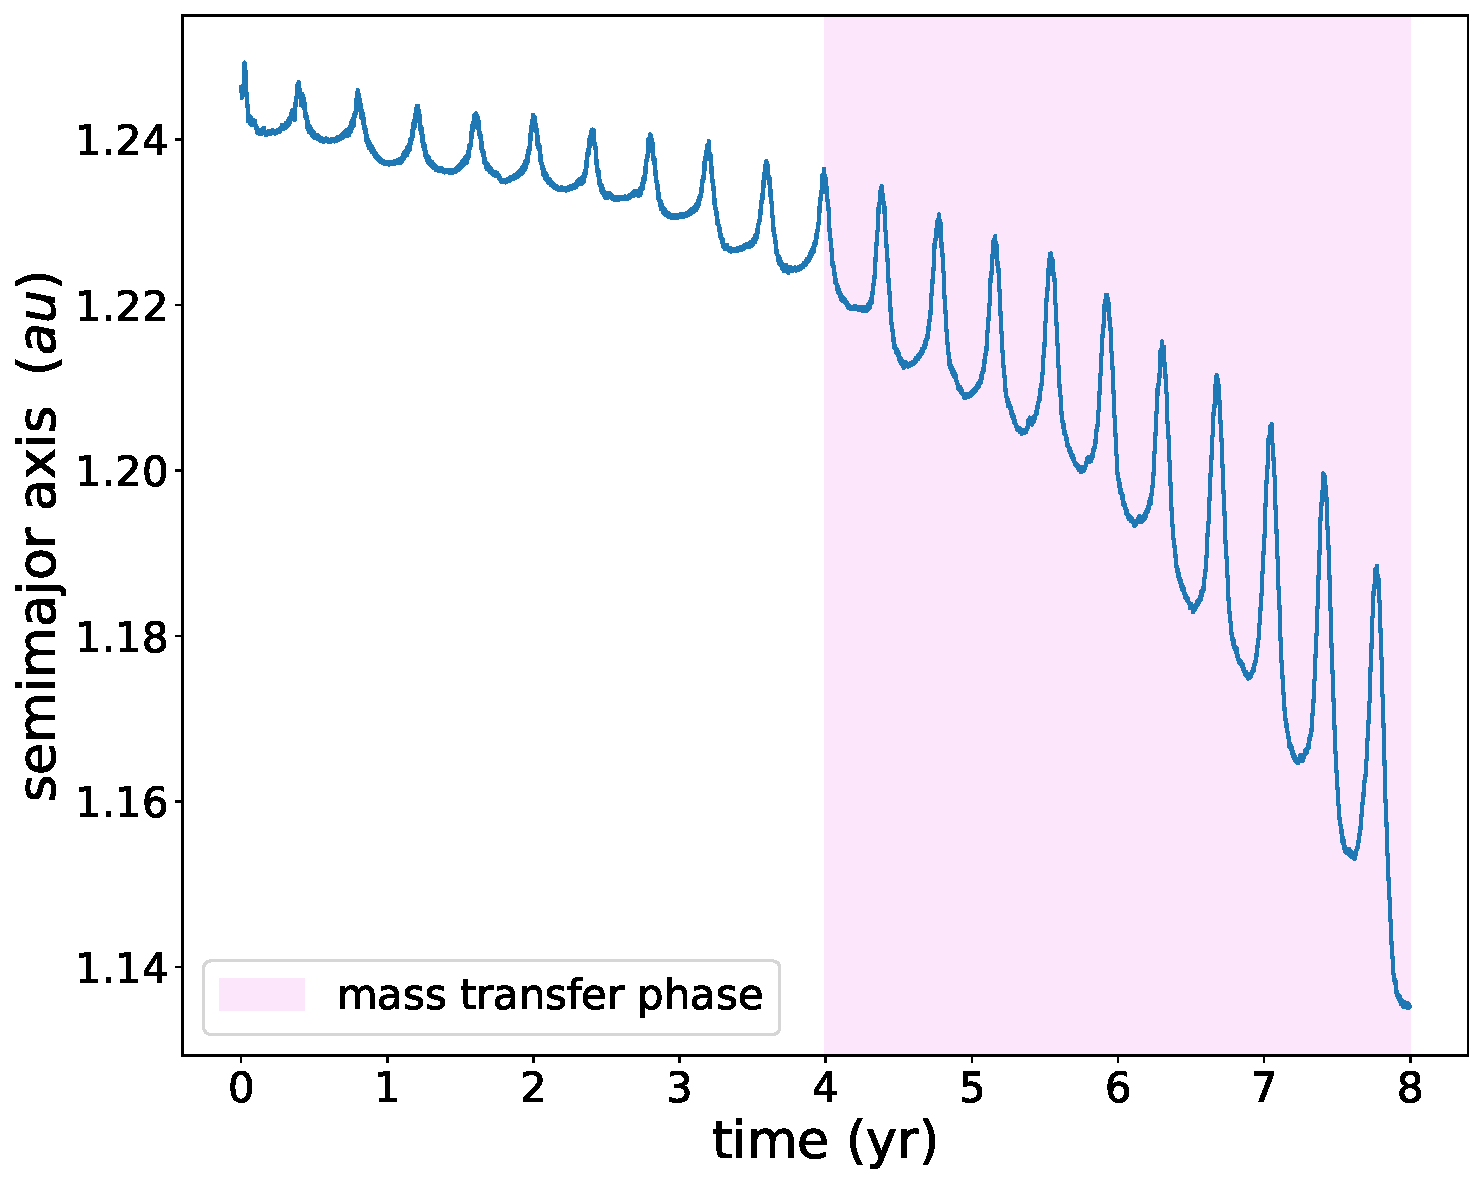
\includegraphics[width=0.9\textwidth]{Thesis/graphs/inc_00/accretion_outer_inc_00_semimajor_axis.pdf}
    \caption{Evolution of the semi-major axis of the outer orbit.}
    \label{fig:accretion_inc_00_outer_semimajor_axis}
\end{figure}
\newpage
\thispagestyle{empty}
\begin{figure}[H]
\vspace{-2cm}
    \centering
    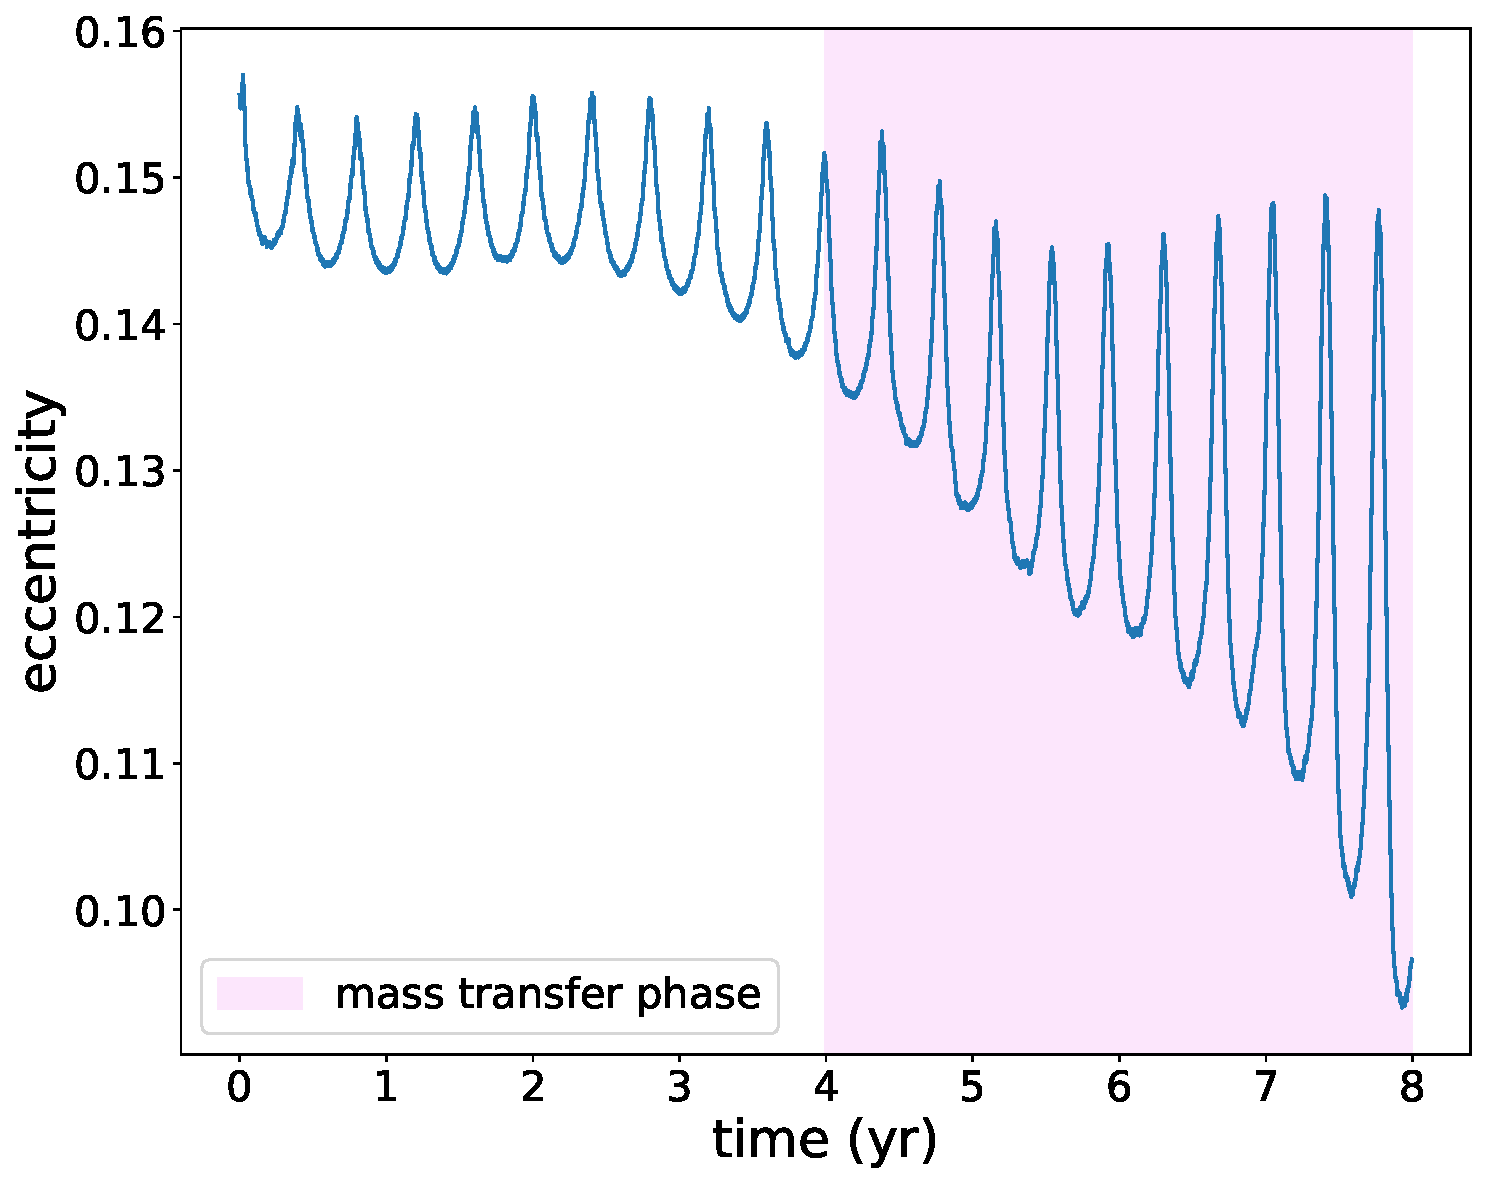
\includegraphics[width=0.9\textwidth]{Thesis/graphs/inc_00/accretion_inc_00_outer_ecc.pdf}
    \caption{Evolution of the eccentricity of the outer orbit.}
    \label{fig:accretion_inc_00_outer_ecc}
\end{figure}
\begin{figure}[H]
    \centering
    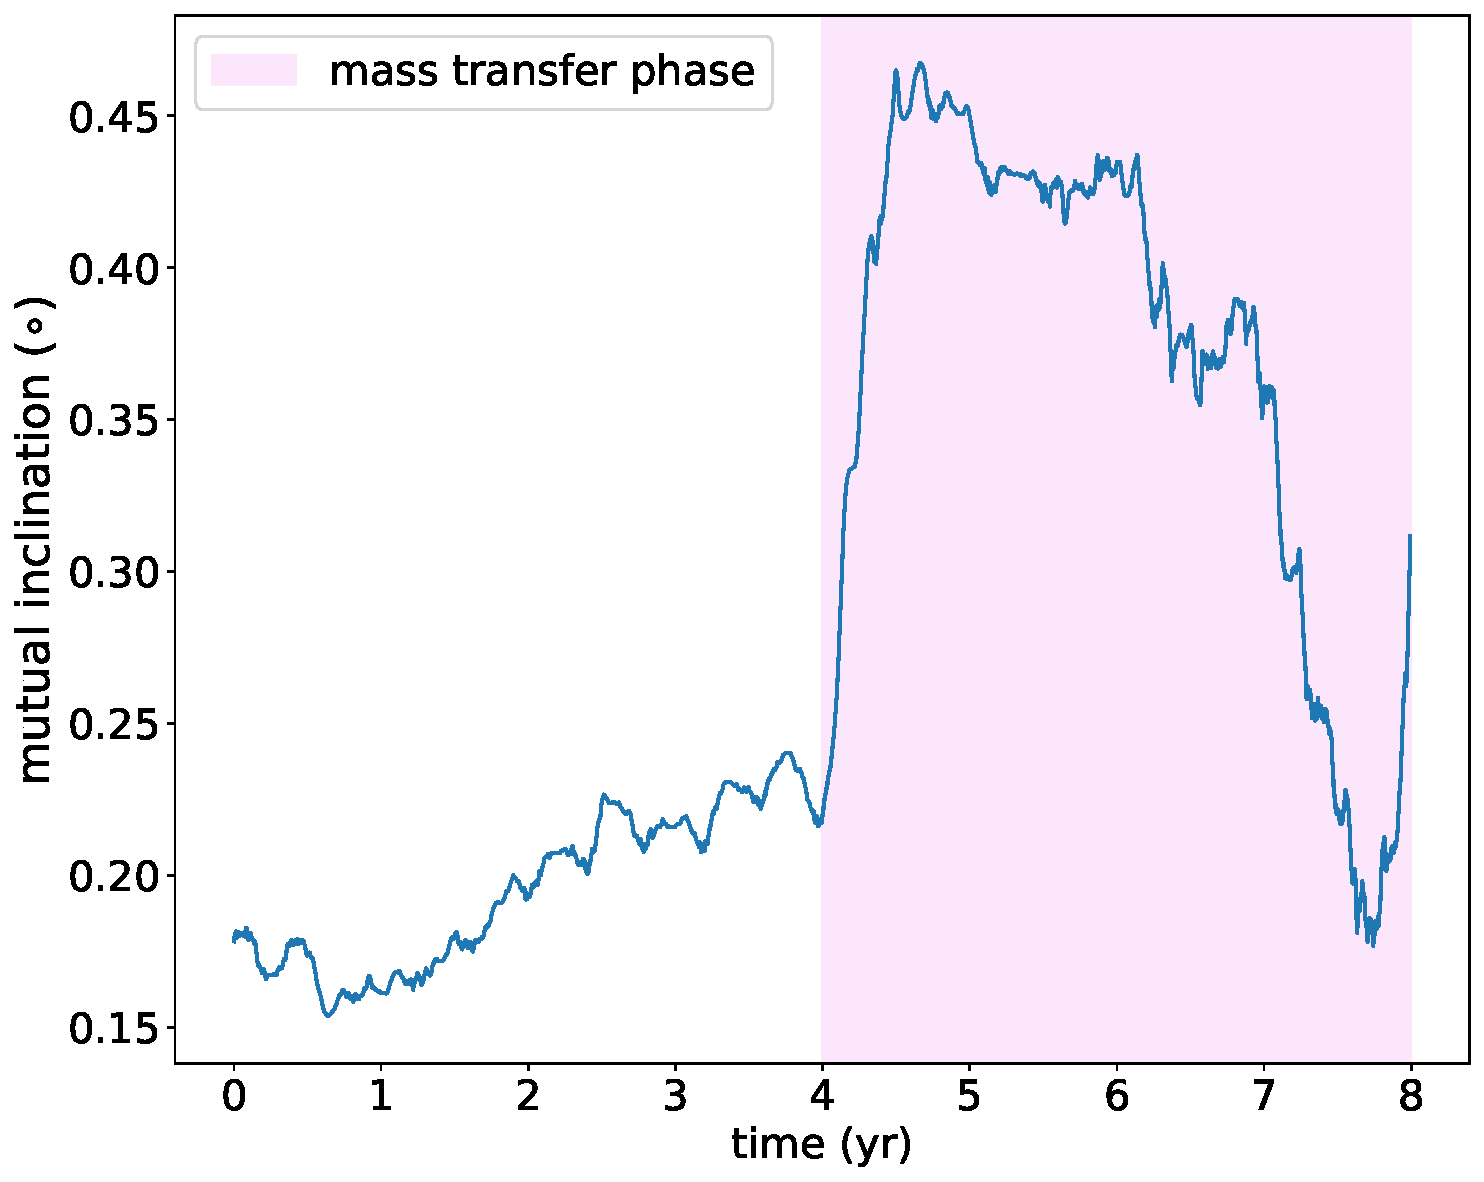
\includegraphics[width=0.9\textwidth]{Thesis/graphs/inc_00/accretion_inc_00_inc.pdf}
    \caption{Evolution of the inclination of the outer orbit relative to the inner orbit.}
    \label{fig:accretion_inc_00_inc}
\end{figure}

Tidal effects between the two orbits dominate the rates of change of orbital parameters up to $t \approx 4$ yr. The spherical symmetry of the giant is disrupted near the pericenter and restored near the apocenter. This series of tidal deformations is a dissipative process that shrinks and circularizes the outer orbit, see white area in \cref{fig:accretion_inc_00_outer_semimajor_axis} and \cref{fig:accretion_inc_00_outer_ecc}.

The effect of mass transfer becomes visible after $t \approx 4$ years. The outer orbit shrinks and circularizes even faster, see blue region in \cref{fig:accretion_inc_00_outer_semimajor_axis} and \cref{fig:accretion_inc_00_outer_ecc}. As mass escapes towards the inner binary, a portion of the transferred mass is accreted by the binary components, while the remainder is expelled from the system. The ejected mass carries away orbital angular momentum and thus the outer orbit decays quicker. Additionally, in the equilibrium-tide model, the circularization timescale is $\propto (\frac{R_{\star}}{\alpha})^{-8}$, hence the faster decay of the orbit ($\alpha$ decreases) leads to a faster circularization too. Finally, there is no clear trend regarding the mutual inclination of the two orbits. However, the outer orbit, which is already coplanar with the inner orbit, remains close to coplanarity. In conclusion,  mass transfer causes the outer orbit to shrink and circularize.

Additionally, as the outer orbit decays, the outer Roche lobe shrinks as well, see \cref{eq:roche_lobe}. Hence, an increasing amount of mass can overflow towards the inner binary and the mass transfer rate becomes progressively higher, see blue region \cref{fig:accretion_inc_00_mass_loss}, leading again to a faster decay of the outer orbit. This runaway effect corresponds to unstable mass transfer.

Despite being out of the scope of this work, it is worth noticing, that shortly after $t=8$ yr, the mass transfer becomes extremely unstable and a triple common envelope is encountered in all cases except for model number 3 listed in \cref{tab:simulations_settings}. For the rest models, the remainder of the tertiary's envelope engulfs the inner binary. In the case of $i_{mut} = 20^{\circ}$, the core of the tertiary is ejected from the system leaving behind a high eccentric binary. Finally, in both cases where the two orbits are initially coplanar, a direct collision completely disrupts the system.


\begin{comment}

Hence, tidal effects between the two orbits dominate the rates of change of orbital parameters up to $t \approx 4$ yr.

It is apparent that the outer orbit tends to become circular and remains coplanar with the inner orbit. Tidal effects between the two orbits dominate the rates of change of orbital parameters up to $t \approx 4$ yr. 
 
\end{comment}

\subsection{Inner orbit}

The mass flowing from the first Lagrangian point of the outer orbit to the inner binary system interacts with the paths of the binary components. As a result, instead of a circumbinary disk, a gaseous cloud, similar to a common envelope (CE) \citep{ivanova2013common}, develops around the binary, see \cref{fig:simualtion_snapshots}.  Part of the mass is accreted by the inner binary and the rest escapes the system through the third Lagrangian point of the outer orbit, see \cref{fig:simualtion_snapshots}. 

In \cref{fig:accretion_inc_00_inner_semimajor_axis} and \cref{fig:accretion_inc_00_inner_ecc}, I present the evolution of the semi-major axis and eccentricity of the inner orbit, 
respectively. Both graphs show the presence of the tertiary, which introduces the observed fluctuations with periods equal to the period of the outer orbit, $P_{out} = 145.5$ day or $P_{out} \approx 0.4$ yr, see subfigure in \cref{fig:accretion_inc_00_inner_semimajor_axis}. Finally, the inner orbit widens, while the effect of mass transfer on the eccentricity of the inner orbit is negligible and the orbit remains circular.
\begin{figure}[H]
    \centering
    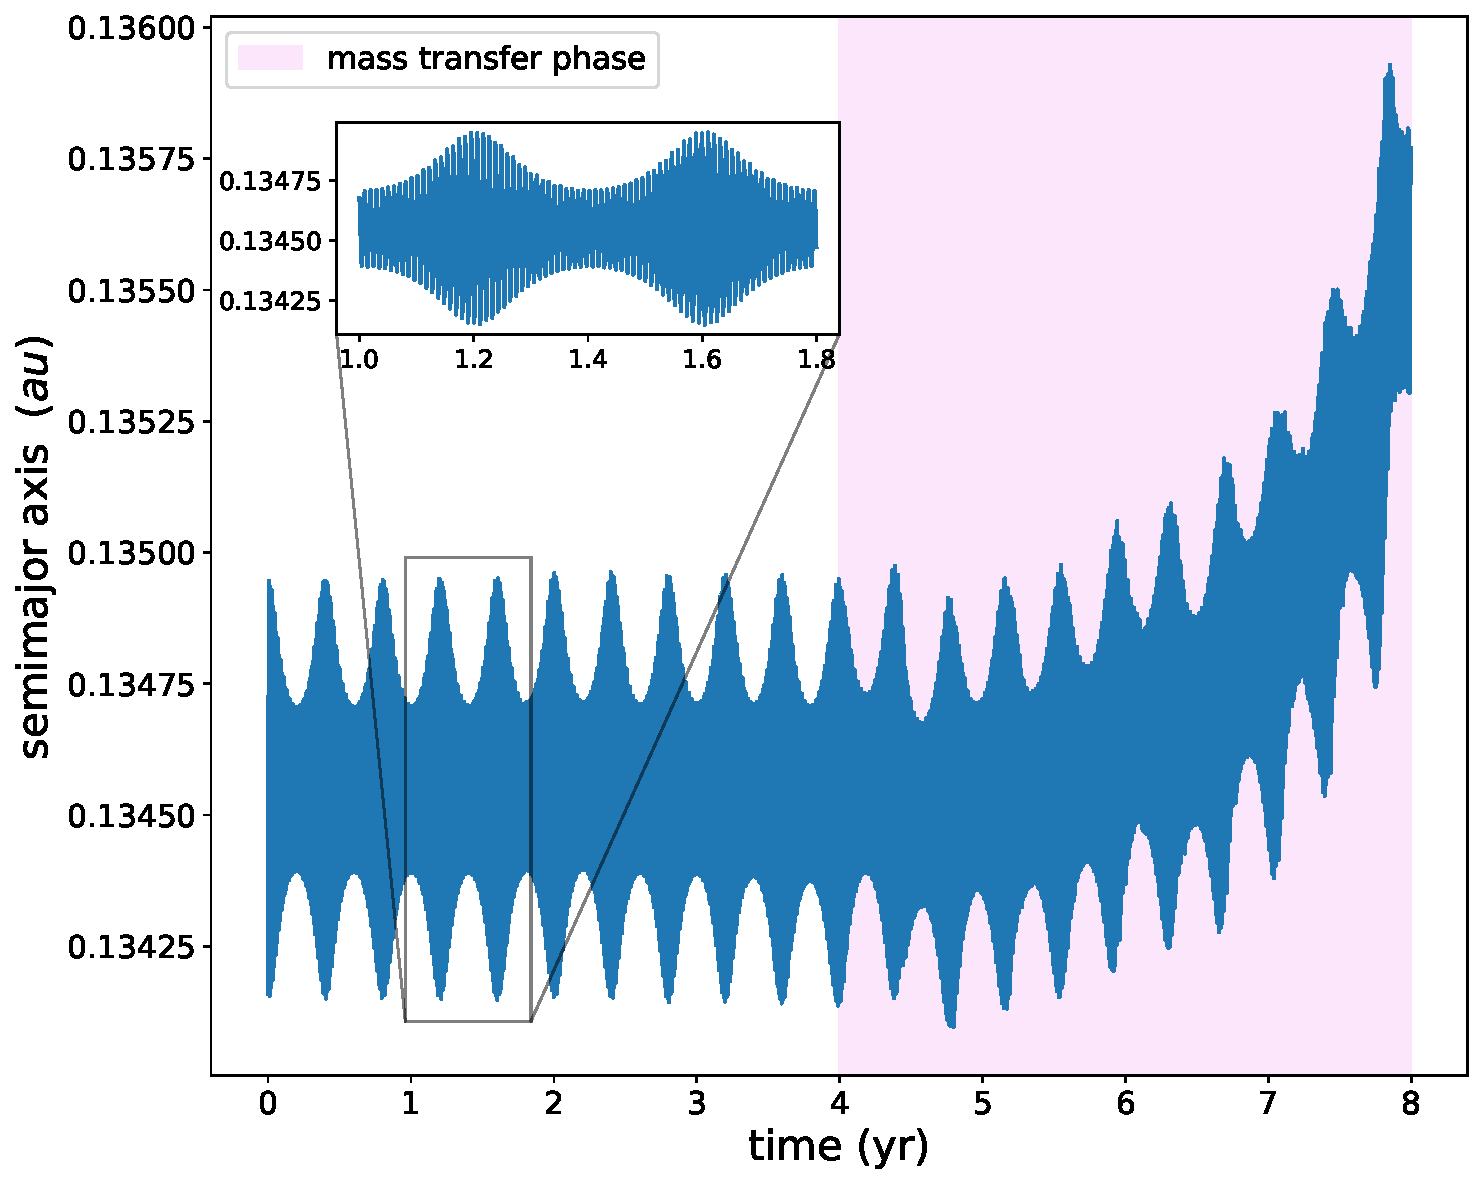
\includegraphics[width=0.9\textwidth]{Thesis/graphs/inc_00/accretion_inc_00_inner_semimajor_axis.pdf}
    \caption{Evolution of the semi-major axis of the inner orbit.}
    \label{fig:accretion_inc_00_inner_semimajor_axis}
\end{figure}
\begin{figure}[!htb]
    \centering
    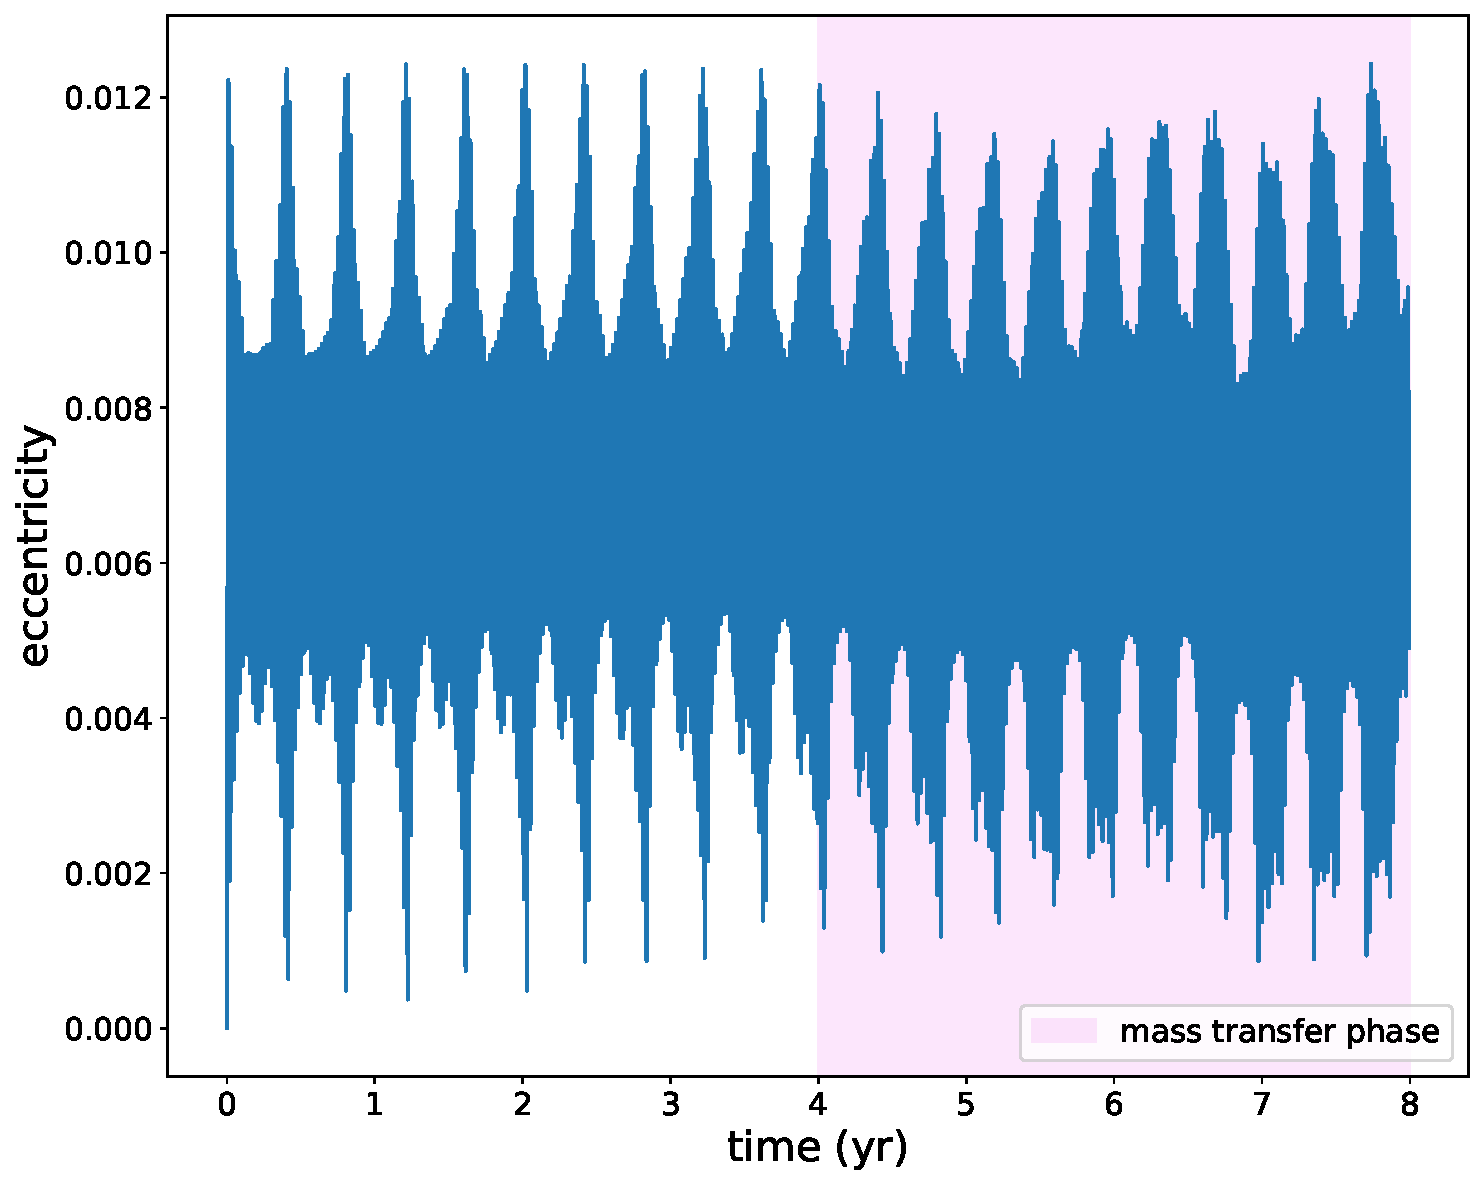
\includegraphics[width=0.9\textwidth]{Thesis/graphs/inc_00/accretion_inc_00_inner_ecc.pdf}
    \caption{Evolution of the eccentricity of the inner orbit.}
    \label{fig:accretion_inc_00_inner_ecc}
\end{figure}

The inner binary is influenced by hydrodynamics, notably gas drag, which in principle always tends to shrink the orbit, as well as the accretion process and the gravitational interaction of the inner orbit with the incoming material stream and the giant's core. The widening of the inner orbit, is a somehow unexpected outcome since a common envelope-like structure around the binary is encountered. On the one hand, in the typical common envelope model, friction between the rotating stars and the slow-rotating envelope is expected to shrink the orbit. On the other hand, this is not a typical common envelope case, thus a detailed discussion regarding this result is taking place in \cref{sec:resolution}. 

%The effect of the later on the evolution of the orbit is complex and depends on the angle at which the mass stream crosses the inner obit. This is discussed in more detail in \cref{sec:inclination}.
